\documentclass[12pt]{article}
\usepackage[a4paper,left=3cm,right=2.5cm,top=3cm,bottom=3cm,]{geometry}
\usepackage{lipsum}
\usepackage[DF,newLogo]{uaThesis}
\def\ThesisYear{2018}
\usepackage{booktabs}
\usepackage{bbold}
\usepackage{float}
\usepackage{afterpage}
\usepackage[english]{babel}
\usepackage{hyperref}
\usepackage{amsmath}
\usepackage{amssymb}
\usepackage{dsfont}
\usepackage[utf8]{inputenc}
\usepackage{geometry} 
\geometry{a4paper} 
\usepackage{graphicx}
\usepackage{amssymb}
 \usepackage{multirow}
\usepackage{comment}
\usepackage{booktabs} 
\usepackage{array}    
\usepackage{paralist} 
\usepackage{verbatim}
\usepackage{subfig}   
\usepackage{fancyhdr} 
\pagestyle{plain}    
\usepackage{sectsty}
\allsectionsfont{\sffamily\mdseries\upshape} 
\usepackage[nottoc,notlof,notlot]{tocbibind} % Put the bibliography in the ToC
\usepackage[titles,subfigure]{tocloft} % Alter the style of the Table of Contents
\renewcommand{\cftsecfont}{\rmfamily\mdseries\upshape}
\renewcommand{\cftsecpagefont}{\rmfamily\mdseries\upshape} % No bold 
%\usepackage{apacite}
\graphicspath{{./Images_Old/}}
\usepackage{tabularx}

\setlength\extrarowheight{2pt}
	
% optional: visual delimiters for floats (figures and tables)
\def\topfigrule{\kern 7.8pt \hrule width\textwidth\kern -8.2pt\relax}
\def\dblfigrule{\kern 7.8pt \hrule width\textwidth\kern -8.2pt\relax}
\def\botfigrule{\kern -7.8pt \hrule width\textwidth\kern 8.2pt\relax}

%nova pagina ao fim da seção
\usepackage{titlesec}
\newcommand{\sectionbreak}{\clearpage}

\begin{document}


\TitlePage
  \HEADER{\BAR\FIG{
\includegraphics[height=60mm]{uaLogoNew.pdf}}} 
         {\ThesisYear}
  \TITLE{João Pedro Dias Rodrigues}
        {Phenomenology of the minimal B - L extension of the Standard Model}
\EndTitlePage
\titlepage\ \endtitlepage % empty page



\TitlePage
  \vspace*{55mm}
  \TEXT{\textbf{o j\'uri~/~the jury\newline}}
       {}
  \TEXT{presidente}
       {\textbf{Margarida Facão}\newline {\small
        Professora Auxiliar do Departamento de Física da Universidade de Aveiro}}
  \vspace*{5mm}
  \TEXT{vogais}
       {\textbf{António Morais}\newline {\small Investigador Pos-doc do Departamento de Física da Universidade de Aveiro}}
  \vspace*{5mm}
  \TEXT{}
       {\textbf{João G. Rosa}\newline {\small
        Investigador Auxiliar do Departamento de Física da Universidade de Aveiro}}
  \vspace*{5mm}
\EndTitlePage
\titlepage\ \endtitlepage % empty page

\TitlePage
  \vspace*{55mm}
  \TEXT{\textbf{agradecimentos~/\newline acknowledgements}}
       {Agradeço principalmente ao meu orientador Dr António Morais pela sua paciência e apoio no decorrer deste semestre.  }
  \TEXT{}
       {Agradeço também à minha família e amigos por toda a motivação e apoio.}
\EndTitlePage
\titlepage\ \endtitlepage % empty page

\TitlePage
  \vspace*{55mm}
  \TEXT{\textbf{Resumo }}
       {Teoria quântica de campo é o nome dado à atualmente aceite teoria quântica que descreve os modelos de interações de partículas e esta é uma combinação da teoria clássica de campo, relatividade restrita e mecânica quântica. O modelo de partículas amplamente aceite para a descrição de partículas é o chamado modelo padrão que em 2012 teve sua ultima partícula descoberta. No entanto, o consenso é também que este modelo está incompleto levando a um vasto interesse em encontrar um novo modelo que explique todas as novas observações experimentais como massas não nulas para neutrinos e a existência de matéria negra.     Motivados por tal,  neste trabalho iremos examinar o modelo padrão e discutir as suas falhas, e feito isto, iremos estudar uma possível extensão conhecida como o modelo B-L-SM. Iremos apresentar como este modelo resolve o problema de massa de neutrinos e que outras diferenças esperamos observar em relação ao modelo padrão. Esta análise não será puramente teórica e, usando uma série de ferramentas computacionais iremos fazer um curto estudo fenomenológico do setor escalar e de gauge do modelo B-L-SM. } 
  \TEXT{}
       {}
\EndTitlePage
\titlepage\ \endtitlepage % empty page

\TitlePage
  \vspace*{55mm}
  \TEXT{\textbf{Abstract}}
       {Quantum field theory is the name of the currently accepted quantum theory that describes models of physical particle interactions. It is a combination of classical field theory, special relativity and quantum mechanics. The currently widely accepted model describing particle interactions is the Standard Model that, in 2012, had its last missing particle discovered. However, the Standard Model is currently thought to be incomplete due to experimental observations like non vanishing neutrino masses and the existence of dark matter. Motivated by this, in this essay, we will examine the Standard Model and discuss its shortcomings with the goal of introducing the B-L-SM model. We will discuss how this model fixes the neutrino mass problem and what other differences we expect to see in relation to the Standard Model. This analysis will not be purely theoretical since we will use an array of computer tools to also study the gauge and scalar sector to the B-L-SM model  }
\EndTitlePage
\titlepage\ \endtitlepage % empty page


\pagenumbering{roman}
\tableofcontents

\cleardoublepage
\listoffigures

\cleardoublepage
\listoftables

\cleardoublepage

\section{Introduction} 
\pagenumbering{arabic}
\setcounter{page}{1}

When the the Large Hadron Collider (LHC) first came online it opened the gate to new discoveries in high energy Particle Physics.
%
Since then it has not only found the last missing particle of the Standard Model (SM), the Higgs boson, but indicated to physicists that there are possibly new horizons for particle physics beyond the SM. 
%
This theory is accurate for most cases, however the current consensus is that it is incomplete. 
%

The experimental data is mounting and the SM is full of inconsistencies,  the most damning evidence against it being the observed spectrum of neutrino masses, the existence of dark matter and the observed matter-antimatter asymmetry.
%
Another telling bit that the SM might be incomplete is the presence an accidental symmetry, and it is now widely believed that extensions to the SM are necessary. 
%
New theories can be formulated that include this additional symmetry, allowing for the solutions to the aforementioned problems.
%
During this essay we will be taking a close look at one of these extensions, the B-L-SM model.

Our goal is then to first introduce the Standard Model, examine its mechanics and then comparing it to the B-L-SM by exploring how and where it differs and how it can address some of the SM shortcomings.  
%
Our analysis will not be only analytical. We will be using a series of computer tools to also study how well our model matches real observed results at particle acceleration and collision experiments like ATLAS.
%
We will follow a bottom up approach and use the $U(1)_{B-L}$ extension of the SM.
%
The model under study will contain an exotic boson denoted as Z prime, which is associated to the addition of a new unitary gauge group.
%
We will later see that this is an extension at the TeV scale, meaning that the new  $U(1)$ gauge field will lead to a mass at the TeV scale proportional to the vacuum expectation value (VEV) af a new scalar that will spontaneously break, $U(1)_{B-L}$. This will be reflected in the mass spectrum of the exotic boson and additional particles stemming from interactions with the broken gauge field.  


\subsection{Basic concepts}

The complexity behind the matters approached in this essay is not to be underestimated, thus we begin with a sizeable review of fundamental concepts.

We will begin by introducing Classical field theory, which can be interpreted as the application of classical dynamics to physical fields and understand how these physical fields interact \cite{schwartz2014quantum}. After which we will introduce the famous Noether's theorem as we begin our study of the concept of symmetry in the context of system dynamics.

\subsubsection{Classical Field Theory} 

To further elaborate on the reasons behind the study of classical field theory, we will introduce this theory as a means to familiarize ourselves with physical fields and their dynamics.  
%
Recall that, from the early quantum mechanical theories, situations like the non-relativistic or relativistic treatment of a ``single particle'' with the Klein-Gordon equation led to a great deal of problems such as negative energy states, a non zero value of the propagator of a particle for a point outside the light cone allowing the particle to break causality.  
%
Quantum Field theory came to later fix these issues through the union of quantum mechanics and classical field theory, creating quantum field theory. 

Moving onwards to definitions, we can conceptualise a physical field as an assignment of a physical quantity to some representation of space. As a quick example of a classical field we can think of the value of temperature in a volume, or as a vector field describing the wind direction and intensity, note how one is a normal vector field and another is a scalar field even though they are both physical fields. 

The first physical theory that can be considered a prime example of classical field theory was Newtons non-relativistic theory of gravity that related a vector field of the force felt on a massive body with mass $m$, $\mathbf{F(r)}$, with the gravitational field created by a massive body with mass $M$, $\mathbf{g(r)}$, which can be written as,
%
\begin{equation}
\mathbf{F}(r) = M \mathbf{\hat{g}(\hat{r}})= - \frac{GMm}{r^2} \mathbf{\hat{r}} \quad , 
\end{equation}
%
where $G$ is Newton's gravitational constant, $\mathbf{\hat{r}}$ is the unitary vector that points from either body to the other and $r^2$ is the square of the distance between both bodies.

\subsubsection{Lagrangian Formalism}
We will begin our discussion of Lagrangian dynamics applied to fields by introducing the action that is written as: 
%
\begin{equation}
\mathcal{S}=\int L \; dt=\int \mathcal{L}(\Phi , \partial_\mu \Phi) \; d^4 x \quad , 
\end{equation}
%
where the Lagrangian, $L$, and the \textit{Lagrangian density}, $\mathcal{L}$ are functions of the field $\Phi $ and its spatial and temporal derivative that can be simplified in covariant notation as $\partial_\mu \Phi$. And note that it's required that the action and by extension the Lagrangian always take real values. 

$\mathcal{S} $ is then defined as a functional of $\Phi$. During this essay we will mostly try to stay faithful to the distinction of Lagrangian and Lagrangian density but these terms are usually used interchangeable and we will later, as an abuse of language use them in that fashion,   
 % 
this action is constrained like in classical mechanics to obey the principle of \textit{least action}, this requires the path taken by a field between an initial and final set of coordinates to leave the action invariant, this can be expressed by:
%
\begin{equation}
\delta \mathcal{S} = 0 \quad .
\end{equation} 
%
This condition can be shown to lead directly to the \textit{Euler-Lagrange} equations,  
%
\begin{equation}
 \partial_\mu \left( \frac{\partial \mathcal{L}(\Phi , \partial_\mu \Phi )}{\partial(\partial_\mu \Phi)} \right) - \frac {\partial \mathcal{L}(\Phi , \partial_\mu \Phi )}{\partial \Phi}  = 0 \quad , 
\end{equation}
%
from where we can extract the equations of motion for the fields.
%
As a example, let's consider a free scalar field. It's Lagrangian density is: \footnote{Note that $\Phi$ could be a complex field and the need for the action to be real makes it so that $\Phi$ must always be multiplied by its conjugate.}: 
%
\begin{align}
\mathcal{L} =\frac{1}{2} \ \eta^{\nu \! \mu} \partial_\mu  \Phi^*  \partial_\nu   \Phi  -  \frac{1}{2}    m^2 \Phi^* \Phi \quad , 
\end{align}
%
the Lagrangian has this form because by definition it is the difference between the kinetic energy of the field, $T$, and the potential energy of the field, $V$, mathematically written as $L=T-V$.
%
Hence the Lagrangian must be this way to ensure the "classical" forms for these quantities.
%
\begin{equation}
T= \int \frac{1}{2} \left( \frac{\partial \Phi}{\partial t} \right)^2 d^3 x \qquad V=\int \frac{1}{2} \left( (\nabla \Phi)^2 + m^2 \Phi^2  \right) d^3 x \quad .
\end{equation}
%
Using then the \textit{Euler-Lagrange} equations we can retrieve the Klein-Gordon equation of motion for this field. 
%
\begin{align}
 (\square + & m^2 )\Phi  =0 \nonumber  \\
 (\square + & m^2 )\Phi^*  =0  \quad , 
\end{align}
%
where we define the d'Alembert operator as $\square=\partial_\mu \partial^\mu$ .

\subsubsection{Transformations, symmetry and Noether's theorem}

A symmetry can be very broadly defined as a property of a system that is preserved or remains unchanged. In physics it's used as a powerful tool that usually helps us to solve problems by allowing for systematic simplifications. 

The most obvious example of symmetry in physics would probably be the discrete rotational symmetry in the shapes of regular crystalline structures, of course in our study matter we aren't really interested in symmetries of \textit{shape}. In our study we will be rather more focused on \textit{internal symmetries} when discussing particle physics \cite{costa2012symmetries}. %perceber melhor% 

Newton was the first to realise that the observation of symmetry in the dynamics of a system or object must not come from a particular solution of the system but by the careful examination of all the possible solutions for the dynamics of a given system, which means that observing a symmetry in the motion of a system must come from the equations of motion and not from a particular solution of those equations. 
%
As an example consider a generic transformation of a field $\phi$,
%
\begin{equation}
\phi \rightarrow \phi + \delta \phi \quad , 
\end{equation}
%
a theory could be called symmetric when such transformation leaves the Lagrangian invariant meaning that $L(\phi)=L(\phi + \delta \phi)$. For example, the complex free scalar field Lagrangian, 
%
\begin{equation}
\mathcal{L} = | \partial_\mu \phi | ^2 - m^2 |\phi|^2 \quad ,
\end{equation}
%
it is invariant under the generic transformation where $\phi  \rightarrow e^{i \alpha } \phi$  for any real $\alpha$. In this complex field $\phi$ we have two different real degrees of freedom since $\phi = \phi_1 + i \phi_2$, but it's more convenient to treat them as $\phi$ and $\phi^*$. The invariance of the Lagrangian preserves the equation of motion since they are directly related as we've seen before. 

The deeper implications of a system having a symmetry were successfully mathematically expressed by Noether with her famous first theorem. Noether's theorem states that the existence of a natural symmetry implies a conservation law and vice-versa any conservation law implies an underlying symmetry.
%
Let's assume we have a generic field $\Phi$ that is transformed in a infinitesimal manner, 
%
\begin{equation}
\Phi(x) \longrightarrow \Phi^\prime (x) = \Phi(x) + \alpha \delta \Phi (x) \quad , 
\end{equation}
%
where $\alpha$ is a constant infinitesimal parameter and $\delta \Phi$ is a deformation of the field. Now to examine any changes made to the dynamics of the system, we do this by imputing the new field into the Lagrangian Density and deriving the new \textit{Euler-Lagrange} equations. We could then say, if the system dynamics remains the same, that this is a \textbf{symmetry} of the system since its dynamics are \textbf{invariant} under these transformations.
%
This is equivalent to stating that the invariance of a system should leave the Lagrangian density invariant up to a 4-divergence, $\mathcal{J}$, because of how the \textit{Euler-Lagrange} equations are formulated. 
%
\begin{equation}
\mathcal{L} \rightarrow \mathcal{L} + \alpha \partial_\mu \mathcal{J}^\mu \quad , 
\end{equation}
%
where the variation of $\mathcal{L}$ i.e $\Delta \mathcal{L}$ can be written as,
%
\begin{align}
\alpha \Delta \mathcal{L} = & \frac{\partial \mathcal{L}}{\partial \phi} \left( \alpha \Delta \phi \right) + \left( \frac{\partial \mathcal{L}}{\partial (\partial_\mu \phi)} \right) \partial_\mu (\alpha \Delta \phi) \nonumber \\
 = & \alpha \partial_\mu \left( \frac{\partial \mathcal{L}}{\partial ( \partial_\mu \phi)} \right) + \alpha \left[ \frac{\partial \mathcal{L}}{\partial \phi} - \partial_\mu \left( \frac{\partial \mathcal{L}}{\partial(\partial_\mu \phi} \right) \right] + \Delta \phi \quad  . 
\end{align}
%
We can clearly see that the second term is the Euler-Lagrange equation so that term vanishes and setting the equation equal to $\alpha \partial_\mu \mathcal{J}^\mu $ we obtain the following 
%
\begin{equation}
\partial_\mu j^\mu (x) \quad \text{for} \quad j^\mu (x) = \frac{\partial \mathcal{L}}{\partial ( \partial_\mu \phi)}  \Delta \phi -\mathcal{J}^\mu  \quad , 
\end{equation}
%
As a note, if we have a symmetry of several fields the first term of $j_\mu$ should be replaced by a sum over those several fields. This $j_\mu$ is the current associated with a symmetry in a system that is conserved through all transformations and for every distinct symmetry we have a different conserved current, so a system with 2 distinct symmetries will have 2 different sets of conserved 4-currents. The charge, $Q_{\text{sym}}$, associated to this current is given by the integral: 
%
\begin{equation}
Q_{\text{sym}} \ = \underset{\text{all \ of \ space}}{\int} j^0 d^3 x \quad ,
\end{equation}
%
so if initially we had a charge inside a volume the only way for us to lose charge over time would be to have a flux of charge leaving the space %and at every point in time this current has it's the volume defined integral value, the \textbf{charge}  
\cite{costa2012symmetries}.

\section{The Standard Model}

The SM is the presently accepted quantum field theory accurately describing strong and electroweak interactions, and has been successfully tested in a number of experiments. 
%
%
The Standard Model is comprised by fermions which are subdivided into quarks and leptons, gauge bosons and a scalar particle, the Higgs boson.
%
\begin{figure}[H]
\centering
  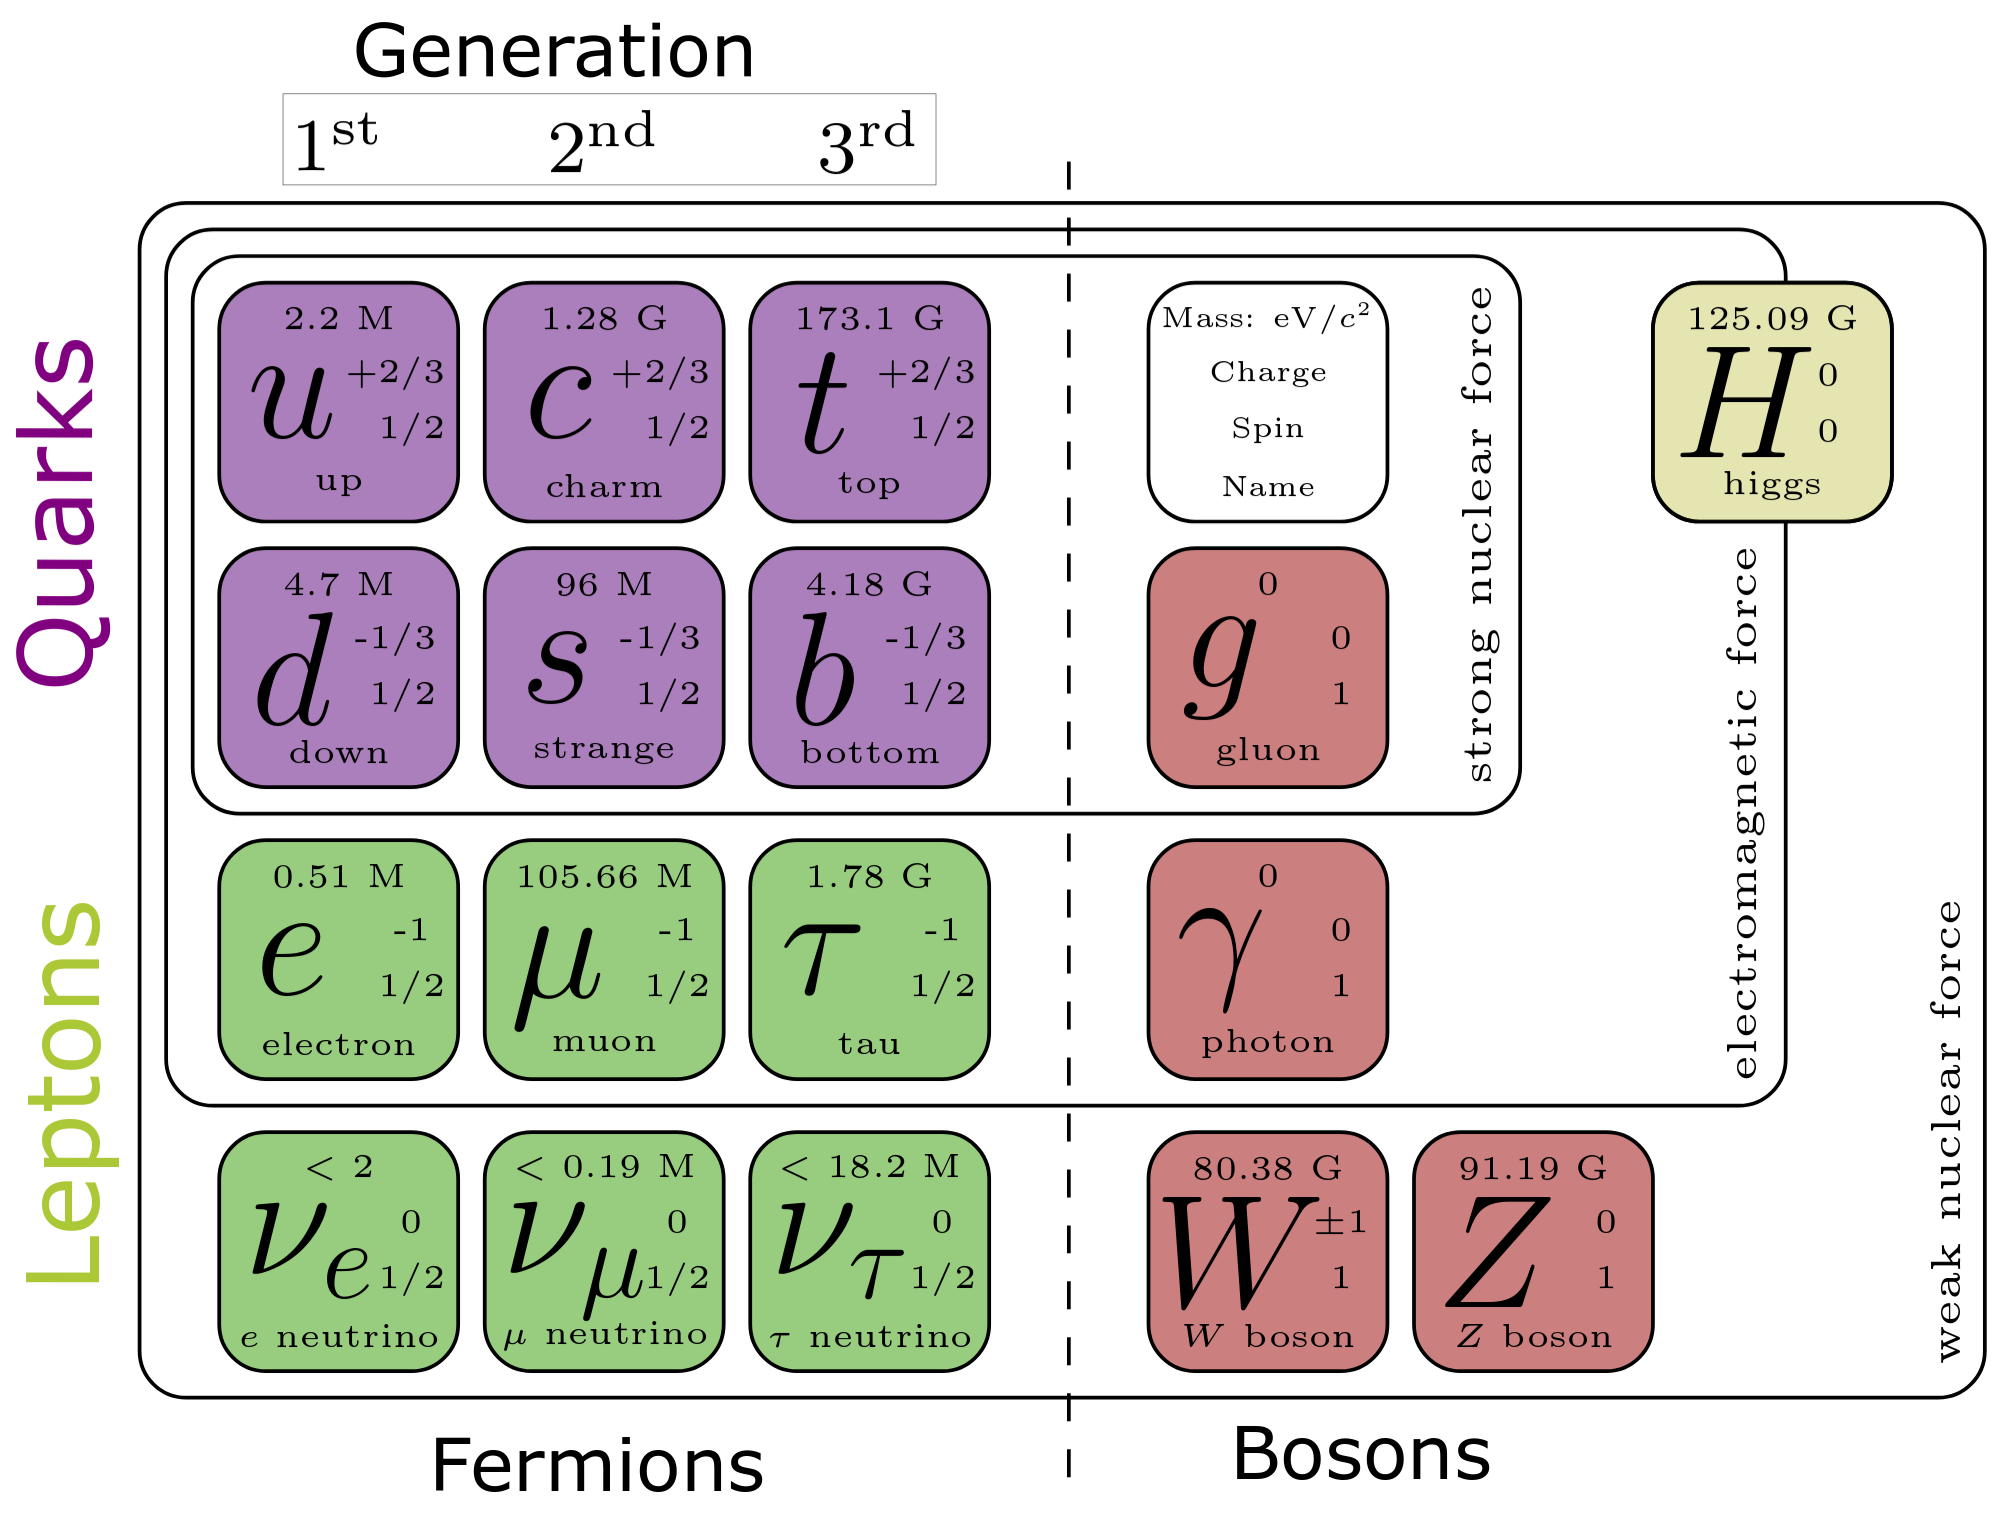
\includegraphics[width=0.7 \linewidth]{SM.png}
  \caption{A diagram of the types and groups of particles that comprise the SM containing information about spin, mass and charge \cite{wiki:sm}.}\label{fig:SMdiag} 
  \end{figure}
%
%As shown in the diagram of Fig. \ref{fig:SMdiag} standard model is composed by a number of bosons types, $Z$, $W^\pm$, gluons (g) and the Higgs boson, $H$, these bosons mediate the 4 fundamental with the $Z$ and $W^\pm$ mediating the weak force, gluons the strong force the photon electromagnetic force and the Higgs field gives particles mass. 
%
As shown in the diagram of Fig. \ref{fig:SMdiag} the Standard Model is composed by force carriers, the weak gauge bosons W and Z, the electromagnetic interaction messenger, the photon, and the strong force mediators, the gluons, as well by matter particles, the quarks and leptons. The Higgs boson is responsible for the mass generation mechanism as we will study in this section.
%
%Fermions, who comprise most of matter, both types of fermions are divided into 3 generations.
 %
Fermions are organized in three generations. Furthermore, there are 6 different types of quarks, up and down for the first generation, charm and strange for the second as well as top and bottom for the third one. Similarly, there are 6 types of leptons, the charged ones, electron, muon and tau, and the associated neutrinos, respectively represented by $(u,d,c,s,t,b)$ while leptons as $(e,\nu_{e},\mu,\nu_{\mu},\tau,\nu_{\tau})$

%These particles are described by spinnors, spinnors that comrpised of fields with difrent dimensions on diferent parts of the SM gauge group. Later we will see these dimensions can change due to Spontaneous symmetry breaking. 
 
So far we have described the physical states that are often denoted as the building blocks of nature. However we have not yet explained how such states have acquired their masses and gauge quantum numbers, such as colour and electric charge. To see this, we start by noting the the SM is a gauge theory based on the group.
%
\begin{equation}
SU(3)_c \times SU(2)_L \times U(1)_Y \quad  .
\label{SMsymmetry}
\end{equation} 
%
Fermions are half integer spin particles most of which have electrical charge (except the neutrinos).  While quarks interact via the weak, electromagnetic and strong forces, the charged leptons only feel the electromeagnetic and weak forces and the neutrinos are solely weakly interacting.  
%
A physical fermion is composed of a left-handed and a right-handed part. While the former transform as $SU(2)_L$ doublets and can be written as
%
\begin{equation}
L^i= \begin{pmatrix}
\nu_{e_L} \\
e_L 
\end{pmatrix},\begin{pmatrix}
\nu_{\mu_L} \\
\mu_L 
\end{pmatrix}
,\begin{pmatrix}
\nu_{\tau_L} \\
\tau_L 
\end{pmatrix} \quad \text{and} \quad Q^i= \begin{pmatrix}
u_{L} \\
d_L 
\end{pmatrix},\begin{pmatrix}
c_{L} \\
s_L 
\end{pmatrix}
,\begin{pmatrix}
t_{L} \\
b_L 
\end{pmatrix} \quad ,
\end{equation}
%
where the $i$ index stands for generation, the latter are $SU(2)_L$ singlets and can be simply represented as
%
 \begin{equation}
e^i_R=\{e_R,\mu_R,\tau_R\}, \quad  u^i_R=\{u_R,c_R,t_R\}, \quad d^i_R=\{d_{e_R},s_{e_R},b_{e_R}\} \quad , 
\end{equation}
%
note also that the quarks form triplets of $SU(3)_C$ whereas leptons are colour singlets. The Higgs boson also emerges from an $SU(2)_L$ doublet with the form,
%
\begin{equation}
H=\begin{pmatrix}
\phi^1 + \; i \; \phi^2 \\
\phi^3 + \; i \; \phi^4  
\end{pmatrix} \quad , 
\end{equation}
%
%
%The Lagrangian that describes all vector particles and gauge fields in the SM can be writen as
%
The full set of gauge quantum numbers in the SM is given in tables \ref{table1} and \ref{table2}. 
%
\begin{table}[H]
\centering
\caption{Gauge bosons and Scalar fields in the SM}
\label{table1}
\begin{tabular}{@{}cccccc@{}}
  \hline	
 Fields & Spin 0 field & Spin 1 Field & $SU(3)_C \times SU(2)_L \times U(1)_Y$  \\
  \hline	
 Gluons  & $\times$  & $g$ & (8,1,0) \\	
A bosons & $\times$  & $A^i$ & (1,3,0)   \\
B bosons & $\times$  & $B$ & (1,1,0)   \\
Higgs field & ($\phi^\pm, \phi^0 )$  & $\times$ & (1,2,1) \\ \hline
\end{tabular}
\end{table}
%
%tenho que perguntar como centrar o 
%
\begin{table}[H]
\centering
\caption{Fermion field dimensions in the SM}
\label{table2}
\begin{tabular}{@{}cccccc@{}}
  \hline	
 Fields & Spin $\frac{1}{2}$ Field & $SU(3)_C \times SU(2)_L \times U(1)_Y$  \\
  \hline	
Quarks (3 gen.) & $Q=(u_L,d_L)$ & $(3,2,\frac{1}{3})$ \\	
$\quad$        & $u_R$ & $(3,1,\frac{4}{3})$   \\
$\quad$   & $d_R$ & $(3,1, -\frac{2}{3})$   \\
Leptons (3 gen.) & $(L=(\nu_{e_L}, e_L )$ & $(1,2,-1)$  \\
$\quad$   & $e_R$ & $(1,1,-2)   $ \\ \hline

\end{tabular}
\end{table}
%
We can then write a Lagrangian invariant under transformations of the $SU(3) \times SU(2) \times U(1)$ as.
%
\begin{align}
\mathcal{L}_{SM} \quad = \quad & (D_\mu H)^\dagger (D^\mu H) - V (H H^\dagger) -  \frac{1}{4} F^i_{\mu \nu} F^{i , \mu \nu} - \frac{1}{4} B_{\mu \nu} B^{\mu \nu} \nonumber \\ 
& + \overline{L_L^i} (i \gamma^\mu D_\mu)  L_L^i +  \overline{Q^i_L} (i \gamma^\mu D_\mu)  Q^i_L +  \overline{L_R^i} (i \gamma^\mu D_\mu)  L_R^i +  \overline{Q^i_R} (i \gamma^\mu D_\mu)  Q^i_R \label{SMfullL}    \\  
 & - [y^d_{jk}\overline{Q}^j_{L} d^k_{R} H +  y_{jk}^u \overline{Q}^j_{L} u^k_{R} \tilde{H} + y^e_{jk} \overline{L}^j e^k_{R} H  + h.c. ] \nonumber \quad , 
\end{align}
%
where $\tilde{H}=i\sigma_2 H$. We define the covariant derivative as, $D_\mu$
%
\begin{equation}
D_\mu = \partial_\mu - i g_S \tau^a G^a_\mu - i g T^i A^i_\mu - i g' Y B_\mu \quad ,  
\end{equation}
%
where $\tau^a= \frac{\lambda_a}{2}$ , $(a = 1, . . . , 8)$ are the generators of $SU (3)_c$, $T_i= \frac{\sigma_i}{2} $, $(i = 1, 2, 3)$ are the generators of $SU(2)_L$ and Y is the generator of $U(1)_Y$. Here the symbols $\lambda_a$ and $\sigma_i$ represent the Gell-Mann and Pauli matrices respectively. 
%The Lagrangian is useal divided in parts to facilitate it's understanding. 
%
%\begin{equation}
%\mathcal{L}=\mathcal{L}_s+\mathcal{L}_{YM}+\mathcal{L}_f+\mathcal{L}_Y
%\end{equation}
%
In the first line of (\ref{SMfullL}), the first term represents the interactions of gauge bosons with the Higgs field and the second term is the scalar potential associated to the said field. 
%
The second line represents the gauge-kinetic terms and gauge boson self interactions. The third line describes the fermion kinetic terms as well as the interactions among fermions and gauge bosons. Finally, the last line shows the Yukawa interactions between the Higgs and the fermions. It is due to the Yukawa interactions that the SM fermions acquire their masses once the electro-weak (EW) symmetry is broken, as we will later see.

%The first term in the first line represents the interactions of gauge bosons with the Higgs and the second term is the scalar potential. The second line represents the gauge-kinetic terms and gauge boson self interactions (for non-abelian ones). The third line describes the fermion kinetic terms as well as the interactions among fermions and gauge bosons. Finally, the last line shows the Yukawa interactions between the Higgs and the fermions and it is due to such interactions that the SM fermions acquire their masses once the EW symmetry is broken.

%The first line is usealy called the scalar sector, $\mathcal{L}_s$ , the second the yang-mills $\mathcal{L}_{YM}$ sector, the third the fermionic sector $\mathcal{L}_f$ and finaly the yukawa sector, $\mathcal{L}_Y$, in the last line. 

Symmetry plays as we will see a key-role in particle physics and given by the field properties we assigned to each field, i.e. the representations of the groups that make up the SM. 
%
The focus of our discussion of the SM is to show how stemming from this we derive the physical particle spectrum that accurately describes reality. 

\subsection{Spontaneous Symmetry Breaking and Goldstone's Theorem} \label{SSBsection}

Having dealt with the fundamentals of field theory and with the concepts of symmetry we find ourselves ready to begin our discussion of the Standard Model. 
%	
However, before jumping into the full details of symmetry breaking in the context of the SM theory, let us look into a simple example, the Abelian Higgs model with a global U(1) symmetry, and stepwise introduce all necessary non-trivial concepts.

%In this sector we will observe the mechanism of spontaneous symmetry breaking, that can be very briefly be described as a "natural" breaking of a symmetry by phenomena in particle physics, we will show it's possible to break a symmetry without adding any terms that would directly break the symmetry. 

%We say that a model contains spontaneous symmetry breaking when the original symmetry (local or global) is pruserved exept for the vacuum state, i.e., the state of minimum energy. On the other hand, if the symmetry was to be explicitly broken we would have to introce extra terms in the Lagrangian that would violate such a symmetry.

%The phenomena that leads to the breaking of the symmetry is the acquisition of a vacuum expectancy value or VEV. In quantum field theory it is possible for a system to have a non zero minimum value that will directly influence the expected value of a field making it non zero as well. 

%This is problematic for symmetry since if a physical fields takes a non zero value might it lead to it taking some sort of orientation. A example of unrelated physical field displaying such behaviour could be exemplified as the magnetic field of a ferromagnetic material, it naturally tends to a configuration with a non zero orientation giving it a natural magnetic field.  

%This directional character of the system's expected value can in some cases break a previously held symmetry by the system this is what is called a case of Spontaneous Symmetry breaking, to examine this we will be starting off with a simple example of a scalar theory. 

Consider the Lagrangian associated to a complex scalar field theory, 
%with $T$ giving it's kinetic energy and $V$ being the associated potential.
%
\begin{equation}
\mathcal{L} =(\partial_\mu \Phi)^* ( \partial^\mu \Phi) -  \mu^2 (\Phi^* \Phi) - \lambda (\Phi^* \Phi)^2 \quad , 
\label{l4}
\end{equation}
%
%
here $\lambda$ is the quartic term is the self interaction that must be a positive value ($\lambda > 0$) to allow for a spectrum of stable bound states and $\mu$ is a real value.
%
This Lagrangian is invariant under global unitary transformations belonging to the $U(1)$ group.
%
\begin{equation}
\phi^\prime \rightarrow e^{i\alpha} \phi \quad  , \quad \phi^{* \prime}=e^{-i \alpha} \phi^* \quad ,
\label{global}
\end{equation} 
%
where $\alpha$ is a real value. This can be easily proven as all terms are even powers of $\phi$
%This is easily be proven due to the fact that all fields are in some form of even power. 
%
\begin{align}
\mathcal{L} =& \frac{1}{2}(\partial_\mu \Phi^{\prime \, *} \partial^\mu \Phi^{\prime} ) -  \mu^2 \Phi^\prime \Phi^{\prime \, *} - \frac{1}{4} \lambda (\Phi^\prime \Phi^{\prime \, *})^2 \nonumber	\\
\mathcal{L} =& \frac{1}{2}e^{i(\alpha-\alpha)}(\partial_\mu \Phi^{*} \partial^\mu \Phi ) -  e^{i(\alpha-\alpha)} \mu^2 \Phi \Phi^* - \frac{1}{4} \lambda (e^{i(\alpha-\alpha)})^2(\Phi \Phi^{*})^2	\\
\mathcal{L} =& \frac{1}{2}(\partial_\mu \Phi^{*} \partial^\mu \Phi^{*} ) - \mu^2 \Phi \Phi^* - \frac{1}{4} \lambda (\Phi \Phi^{*})^2	 \quad . \nonumber 
\end{align} 
%
The next step is to examine the potential portion of the Lagrangian, 
%
\begin{equation}
V(\Phi)=  \frac{1}{2} \mu^2 \Phi \Phi^* + \lambda (\Phi \Phi^{*})^2 \quad , 
\end{equation}
%
and determine its minima by solving:
\begin{equation}
\frac{\partial V(\Phi)}{\partial | \Phi | } = 0  \quad .
\label{minvalpot}
\end{equation}
%
Analysing the lower energy states we note that in the case of $\mu > 0$ the potential is simply a parabola with its minima sitting at the origin.
%
However were we to say $\mu$ is a negative number (\ref{minvalpot}) changes to,	
%
%something very interesting would happen, the minimum condition would be calculated by the expression,
%
\begin{align}
2  \mu^2 |\Phi|+ 4 \lambda |\Phi|^3 & = 0  \quad , 
\end{align}
%
from this equation we conclude that,
%And now it returns a negative number as the potentials minima and the former minima, zero, now became a relative maximum.  We could equate the minima equation as,
%
\begin{equation}
|\Phi_{min}|^2 = -\frac{\mu^2}{2 \lambda} = v^2  \quad .
\end{equation}
%
The value of the scalar field in the vacuum is non-vanishing and is denoted as vacuum expectation value, or VEV for short. 
%Whose conditions can be written as continuous set of solutions in radial form, 
%
We can parametrize the field at the minimum by rewriting it in radial form, 
%as the value of the field in the minimum as
%
\begin{equation}
\Phi_{min} = | \Phi_{min} | e^{i \gamma} \quad , 
\end{equation}
%
which represents a set of degenerate vacuum states.
%
% to the observant eyes it's clear one symmetry of the potential is now broken by this change, we can see by examining both the potentials that in both cases we have phase invariance but in the case where $\mu$ is negative we no longer have a directional radial invariance around the VEV. This is the graphical representation of a case of spontaneous symmetry breaking or SSB. 
%
Comparing both cases, for positive and negative values of  $\mu^2$, we see that for the latter case, while a phase invariance is still preserved we no longer have a directional radial invariance about the VEV. So the previously held symmetry was spontaneously broken (SSB) and a graphical representation of this can be seen in Fig. \ref{phase}.

%We can see this easily if we shift the field into the minima, and considering the phase is irrelevant we will take the particular solution where $\gamma$ is zero to simplify the mathematics. So the shift can be written as transforming the previous field. 

Defining $| \Phi_{min} | = v$ we can write and study the scalar field in the vacuum by performing the shift,
%
\begin{align}
\Phi(x) & \longrightarrow \Phi^\prime (x) \nonumber \\ 
\frac{1}{\sqrt{2}} \left( \phi_1 (x) + i \phi_2 (x) \right) & \longrightarrow  \frac{1}{\sqrt{2}} \left( \eta(x) + v + i \epsilon(x) \right)  \quad , 
\end{align}
%
Where $v$ is equal to $\sqrt{-\frac{\mu}{\lambda}}$. Now plugging this new field into the Lagrangian must return an equivalent physical description of the dynamics of the system, now expressed as,
%
% of dynamics, we simply changed the fields in which these are expressed, $\mathcal{L} \equiv \mathcal{L}^\prime$.  
%
\begin{equation}
 \mathcal{L} = \frac{1}{2} \partial_\mu \epsilon(x) \partial^\mu \epsilon(x) + \frac{1}{2}\partial_\mu \eta(x) \partial^\mu \eta(x)  - \frac{1}{2} ( 2\mu ^2)  \eta^2 - \frac{1}{4} \lambda (\epsilon^2 + \eta^2)^2 - \lambda  v  (\epsilon^2 + \eta^2) \eta \; .
\end{equation}
 
Comparing this new Lagrangian density and the former we see that while in the former we had a squared mass term with value $\mu^2$ for both $\phi_1$ and $\phi_2$, now in this new redefinition we only have one mass term in $\eta$ with squared mass equal to $ m^2_\eta = - 2 \mu^2 = 2 \lambda v $ and a massless scalar field $\epsilon$.
%
The physical meaning of these fields is that $\eta$ represents the quantum fluctuations above the constant vaccum value along the radial direction and the field $\epsilon$ represents the fluctuations along the angular directions.% the fact that the potential doesn't change along this type of movement being reflected by it being a massless scalar field. 
%
The fact that the potential doesn't vary along the latter direction is reflected in a massless scalar field. Note that, whenever we have a continuous symmetry that is spontaneoulsy broken, there will be as many massless scalar particles as the number of broken generators. This results is know as the \textit{Goldstone Theorem} and such massless degrees of freedom are denoted as Goldstone bosons. For our particular case, the only single generator of the $U(1)$ symmetry is sponteneoulsy broken, which yields one massless Goldstone boson that we have identified with $\epsilon$.

Note that, when the sign of $\mu$ squared goes from positive to negative the system goes through a phase transition where the original symmetry is spontaneously broken in the vacuum states. This is graphically represented in Fig.\ref{phase}.

%In summation what we just observed discussed is that when $\mu$ changes from a positive number to a negative number what we observe is that the system goes trough a phase transition. A phase transition where a previous existing symmetry, in this case  $U(1)$, is broken as a consequence of such breaking previously conserved quantities stemming from a application of noether's theorm are still conserved but actions from the groups whose symmetries originated these quantities no longer leave the system invariant.  

\begin{figure}[H]
\centering
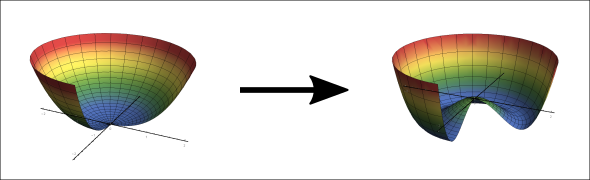
\includegraphics[width=14cm, height=4.5cm]{Des.png}
\caption{Phase Shift of the Potential in a Higgs Style Field}
\label{phase}
\end{figure}

%This change that $\mu$ goes trough, going from positive to negative is quite similar to what happens as a  consequence of the renormalization procedure for the Higgs field a process that we will explore later and that leads to the mass generation for the electroweak $W^\pm$ and $Z$ bosons in the standard model, represented graphically in the figure \ref{phase}.

%The massless particle that appeared in this case are a direct consequence of Goldstone's theorem and is usually called a Goldstone boson. The theorem states in a system with a certain number of linearly independently continuous symmetries that has a number of these spontaneously  broken the same number of  massless particles will appear in the system. 

\subsection{Gauging U(1): The example of Quantum Electrodynamics}

In the previous section we discussed the particular case of a complex scalar field transforming under a global symmetry.
% where the entirety of the field was changed by a constant phase given by $\alpha$.
%
%This symmetry would imply that the choice of phase is irrelevant when studying the field. The objective of this chapter is to show that by restraining this phase change to be coherent with the limitations of relativistic theories, this is that the phase of a field, like all information, can't be changed everywhere instantly, translating in the act of changing a phase of a field now being a transformation that isdone locally with $\alpha$ being no longer being constant but a function of space-time.  
%
%To evade the goldstone theorem in these cases and to maintain the phase invariance under such transformations, what known formally as promoting the global symmetry to a local symmetry, leads us into gauge theories. 
%
%In gauge theories we add fields known as gauge fields that interact with scalar fields and maintain the discussed phase symmetry ($U(1)$). 
%
%It can then be shown that electromagnetism stems naturally from gauge fields connected to scalar fields, examine the following local transformations that replaced \ref{global}. 
%
Let us now consider a local transformation by replacing the phase in (\ref{global}) by a space-time dependent phase $\alpha (x)$

%
\begin{equation}
\phi(x) \rightarrow e^{i q \alpha (x)} \phi (x) \quad , \quad \phi^*  (x)\rightarrow e^{-i q \alpha (x)} \phi^* (x)  \quad ,
\end{equation}
%
Introducing this transformation, where $q$ is the charge associated to the symmetry, to the former Lagrangian density (\ref{l4}), we can see that all but the derivative terms are invariant. Those particular terms now take the form,
%
\begin{align}
\partial_\mu \Phi^\prime \rightarrow &  \partial_\mu \left(e^{i \alpha(x)} \Phi \right) = e^{i \alpha \left(x\right)}.\left(  i \; \Phi (\partial_\mu \alpha )   + \partial_\mu \Phi \right) \\
\partial_\mu \Phi^{\prime \ *} \rightarrow &  \partial_\mu \left( e^{-i \alpha \left(x \right)} \Phi^* \right) =  e^{-i \alpha \left(x \right)}.\left(  -i \; \Phi^* (\partial_\mu \alpha )   + \partial_\mu \Phi^* \right) \quad , 
\label{deriv}
\end{align}
%
meaning the Lagrangian is no longer invariant. In fact we note it changes by, 
\begin{equation}
\delta \mathcal{L} =   i \; q \Phi (\partial_\mu \alpha )  \Phi^* - i \; q \partial_\mu \Phi \Phi^* (\partial_\mu \alpha ) + \Phi \Phi^* q^2 \partial_\mu \alpha \partial^\mu \alpha    \quad . 
\end{equation}
%
To reattain invariance under local gauge transformations we have to introduce a new 4-vector $A_\mu$, denoted as the gauge field in what follows, as well as three new terms in the Lagrangian allowed by the gauge symmetry. We also note that the gauge field has to transform in such a way to cancel the effects coming from the derivative terms in \ref{deriv} and has the form
%
%We then specify that this field has to be transformed in such a way that will conserve the symmetry by countering the effects seen on the kinetic derivative terms, leading to the transformation seen in,
%
\begin{equation}
 A_\mu + \frac{1}{q} \partial_\mu \alpha \left(x \right)=A_\mu^\prime \quad , 
\end{equation} 
%
The new added terms are then,
%
\begin{align}
\mathcal{L}_1 & =  - i \; q \left( \Phi^* \partial_\mu \Phi  - \Phi \partial_\mu \Phi^* \right) A_\mu \\
\mathcal{L}_2 & =  q^2  A^\mu A_\mu \Phi \Phi^*  \quad , 
\end{align}
%
%Here $\mathcal{L}_1$ is added to retain invariance and since we coupled the gauge field to the scalar fields we must also add the interaction term seen in $\mathcal{L}_2$ 
%
In addition to these terms we add another term to the Lagrangian, $\mathcal{L}_3$, containing kinetic terms for the gauge field and invariant under the transformation (\ref{deriv}) and reads,
%
\begin{align}
\mathcal{L}_3 & = -\frac{1}{4} \left[ \left( \partial_\mu A_\nu - \partial_\nu A_\mu \right) \left( \partial^\mu A^\nu - \partial^\nu A^\mu \right) \right] , \nonumber \\ \mathcal{L}_3  &= \frac{1}{4} F_{\nu \mu}(x)  F^{\nu \mu}(x) \;  , 
\end{align}

% that is responsible for gauge invariance connected to the field transformation and is the curl of the gauge field, $F_{\mu \nu}$. 
Puting all together we get,
%
 \begin{align} 
  \mathcal{L}_{tot}= & \mathcal{L}_0+\mathcal{L}_1+\mathcal{L}_2+\mathcal{L}_3 \nonumber \\
  \mathcal{L}_{tot}= & (\partial_\mu \Phi)(\partial^\mu \Phi^*) - iq(\Phi^* \partial^\mu \Phi - \Phi \partial^\mu \Phi^* )A_\mu + q^2 A_\mu A^\mu \Phi^* \Phi - m \Phi^* \Phi - \frac{1}{4} F^{\mu \nu} F_{\mu \nu} \nonumber \\ 
  \mathcal{L}_{tot}= & (\partial_\mu \Phi + iq A_\mu \Phi)(\partial^\mu \Phi^* - iq A^\mu \Phi)- m^2 \Phi^* \Phi  - \frac{1}{4} F^{\mu \nu} F_{\mu \nu} \nonumber \\
  \mathcal{L}_{tot}= & D_\mu \Phi D^\mu \Phi^*  - m^2 \Phi^* \Phi  - \frac{1}{4} F^{\mu \nu} F_{\mu \nu} \quad ,  \label{totgarbage}
 \end{align}
%
which preserves the original structure but with normal derivatives replaced by what we denote as covariant derivatives. Note that it is in the terms involving the covariant derivatives that we have interactions involving the gauge and the scalar fields.
 
%As a side note, $F_{\mu \nu}$ is the electromagnetic field tensor, we have just shown that the electromagnetic Field appears seamlessly from the interaction between a scalar field and a gauge field that conserves the phase symmetry in a relativistic context. 



\subsection{The Higgs mechanism and the mass generation of the Gauge bosons}

%Of the Gauge group we just defined we will spawn 4 gauge fields named $A_\mu^i$ and $B_\mu$ corresponding respectively to the generators $I^i$ and $Y$. Through observations it was shown that these interact in a very short range requiring them to be massive vector bosons to mathematically describe the proper behaviour. 

%The solution that lead to the attribution of mass to these bosons came trough the mechanism of spontaneous symmetry breaking applied to the Higgs field, and allowed for these 4 fields to be identified as the $W^\pm$ and $Z$ bosons after mixing with goldstones created by the broken symmetries, since the one boson must remains massless, the photon $A^\mu$,we know that only 3 symmetries must be broken, given this the minimal choice for the Higgs field would be a complex scalar doublet $\phi$ represented as 
%\begin{equation}
%\phi = \left( \begin{matrix}
%\phi^+ \\
%\phi^0 
%\end{matrix} \right)
%\end{equation}
%Where the "top"? part of the field is dedicated the to elements with charge while the lower part is neutral. 

%This field has weak isospin charge $I$ of $\frac{1}{2}$ and a hypercharge value of of $1$. This choise allows the breaking of the $SU(2)_L$ group and the $U(1)_Y$ group. The gauge sector in the SM is given by the Lagrangian

Coming back to the SM as defined above, we can now study the mechnism of spontaneous symmetry breaking. Let us then consider the part of the Lagrangian containing the scalar covariant derivatives as defined in eq. (\ref{SMfullL}) , the scalar potential and the gauge-kinetic terms:
%
\begin{equation}
\mathcal{L}_{gauge} = (D_\mu H)^\dagger (D_\mu H) - V (H H^\dagger) - \frac{1}{4} F^i_{\mu \nu} F^{i , \mu \nu} - \frac{1}{4} B_{\mu \nu} B^{\mu \nu} \quad , 
\label{iamgarbagemanyes}
\end{equation} 
The elements of this sector are defined as,
\begin{equation}
V(H H^\dagger ) = \mu^2 H^\dagger H + \lambda (H^\dagger H)^2 \quad , 
\end{equation}
\begin{equation}
 F^i_{\mu \nu}= \partial_\mu A^i_\nu - \partial_\nu A^i_\mu + g \epsilon_{ijk} A^j_\mu A^k_\nu  \quad , 
\end{equation}
%
In this formulation the constants $g$ and $g^\prime$ are the gauge couplings of the groups $SU(2)_L$ and $U(1)_Y$. 
% 
As the potential is identical to the one dicussed in Sec. \ref{SSBsection}, we know that we have a phase shift, namely $\mu^2 < 0$ and what kind of VEV we are expected to find, namely
%
\begin{equation}
(H^\dagger H) = \frac{-\mu^2}{2\lambda} = \frac{1}{2} v  \quad , 
\end{equation} 
%
%Given that electrical charge must be conserved only the lower part of the field can be given a non-vanishing vev and it's indeed convenient to shift the field to the following minima choise, 
The vacuum can be aligned in such a way that we have
\begin{equation}
H_{min} = \frac{1}{\sqrt{2}} \begin{pmatrix} 0 \\
v 
\end{pmatrix} \quad .
\end{equation}
This vacuum will break the $SU(2)_L \times U(1)_Y$ symmetry down to $U(1)_Q$. this means that in the begining there are four generators, which are $T^{1,2,3}$ and $Y$, and after the breaking we are solely left with one unbroken combination that is $Q =  (T^3 + 1/2)$. This means that in total we will have three broken generators, thus, from Goldstone Theorem, there will be three massless particles. 

As we have seen for the abelian Higgs model, the Goldstones modes can be parameterized as phases in the field space and then can be "rotated away" in the physical basis, leaving us with a single physical massive scalar, the Higgs boson. Note that, with this transformation we are removing three scalar degrees of freedom.  However, they cannot just disappear from the theory and will be absorbed by the massive gauge bosons.
%
In fact, a massless gauge boson contains only two scalar degrees of freedom (transverse polarization). Meanwhile, a massive vector boson has two transverse and a longitudinal polarization, i.e., three scalar degrees od freedom. So, as we discussed above, while before the breaking of the EW symmetry we have four massless gauge bosons, after the breaking we are left with three massive ones. This means that there are three extra scalar degrees of freedom showing up in the gauge sector. It is then commonly said that the goldstone bosons are ``eaten" by the massive gauge bosons and the total number of scalar degrees of freedom in the theory is preserved. Therefore, without loss of generality, we can rewrite the Higgs doublet as

\begin{equation}
 \begin{pmatrix}
G_1 + i G_2 \\ 
v + h(x) + i G_3 
\end{pmatrix} = H (x) \rightarrow H (x) =  \frac{1}{\sqrt{2}} \begin{pmatrix}
0 \\ 
v + h(x) 
\end{pmatrix} \quad .
\label{shame}
\end{equation}
Once the Higgs doublet acquires a VEV, the Lagrangian (\ref{iamgarbagemanyes}) can be recast as:
\begin{align}
\mathcal{L}^\prime = & \frac{1}{2} \partial_\mu h \partial^\mu h - \frac{1}{2} (2v^2 \lambda) h^2
 - \frac{1}{4} F^i_{\mu \nu} F^{i , \mu \nu} - \frac{1}{4} B_{\mu \nu} B^{\mu \nu}  \nonumber \\
& + \frac{1}{8} v^2 g^2 (A^1_\mu A^{1,\mu}+ A^2_\mu A^{2,\mu}) +  \frac{1}{8} v^2  (g^2  A^3_\mu A^{3,\mu} + g^{\prime 2} B_\mu B^\mu - 2 g^2 g^{\prime 2} A^3_\mu B^\mu ) \quad , 
\label{complicatedpart}
\end{align}
A few things become obvious first, we have a lot of mass terms most stemming from the squared gauge fields and a lonesome squared mass term belonging to the real scalar field we know to be the Higgs field. This makes the Higgs boson mass in the SM to be given by,
%
\begin{equation}
M_h= (2v^2 \lambda) \quad .  
\end{equation}
%
To obtain masses for the gauge bosons we need to rotate the gauge fields to a basis where the mass terms are diagonal. First, it is straightforward to see that the electrically charged eigenstates are given by %\ref{gagestate}
%First the fields that carry defined charge that can be easily shown to be 
\begin{equation}
W^\pm_\mu = \frac{1}{\sqrt{2}} (A^{(1)}_\mu \pm i A^{(2)}_\mu) \quad , 
\label{gagestate}
\end{equation}
meaning that the mass of the W bosons is, 
\begin{equation}
M_W= \frac{1}{2} v g \quad .
\end{equation}
The situation becomes a bit more complicated for the second term in (\ref{complicatedpart}) due to a mixing between $A_\mu^3$ and $B_\mu$. In the gauge eigenbasis the mass terms read
\begin{equation}
\begin{pmatrix}
A_\mu^3 && B_\mu
\end{pmatrix} \cdot  \frac{1}{4} \nu ^2 \begin{pmatrix}
g^2  & -g g^\prime \\
-g g^\prime & g^{\prime 2} 
\end{pmatrix} \cdot \begin{pmatrix}
A_\mu^3 \\  B_\mu
\end{pmatrix}  \quad , 
\end{equation} 
which can be diagonalized to obtain
\begin{equation}
\begin{pmatrix}
A_\mu && Z_\mu 
\end{pmatrix} \begin{pmatrix}
0  & 0 \\
0  & \frac{1}{2} v \sqrt{g^2 + g^{\prime 2}} 
\end{pmatrix}  \begin{pmatrix}
A^\mu \\ Z^\mu
\end{pmatrix}  \quad , 
\end{equation}
%Where the new eigenvectors that represent the $Z$ boson and the photon, $A^\mu$ in terms of the former base are written as,
%
we identify the eigenvector associated to the eigenvalue 0 to the photon and the massive one, $ M_Z =  \frac{1}{2} v \sqrt{g^2 + g^{\prime 2}} $, to the Z boson. Such eigenvectors can be written as
%
\begin{align}
A_\mu &=\cos(\theta_\omega) B_\mu + \sin(\theta_\omega) A_\mu^3 \quad ,  \\  
Z_\mu & =- \sin(\theta_\omega) B_\mu + \cos(\theta_\omega) A_\mu^3 \quad , 
\end{align}
%
where $\theta_w$ is the so called Weinberg mixing angle and is defined as
\begin{equation}
\cos(\theta_\omega)=\frac{g}{ \sqrt{g^2 + g^{\prime 2}}} \quad , 
\end{equation}
thus clearly showing the massless photon along with a massive Z boson with mass $M_Z= \frac{1}{2} \nu \sqrt{g^2 + g^{\prime 2}} $. 
%
So we conclude our exploration of the electroweak sector with all the correct massive spectrum observed and its origin discussed.


\subsection{The fermion sector on the Standard Model}

In order to generate mass for the fermions we can have a closer look at the last line in eq. (\ref{SMfullL}). If we replace the Higgs by the shift in Eq. (\ref{shame}) we get, 
%
%\begin{equation}
%\mathcal{L}_y = y^d_{jk}\overline{Q}^j_{L} d^k_{R} (\nu + h(x)) +  y_{jk}^u \overline{Q}^j_{L} u^k_{R} (\nu + h(x)) + y^e_{jk} \overline{L}^j e^k_{R} (\nu + h(x)) 
%\end{equation}
%
\begin{align}
\mathcal{L}_y = & y^d 
\begin{pmatrix}
\overline{u_L} & \overline{d_L} 
\end{pmatrix} d_R 
\begin{pmatrix}
0\\ v + h(x)
\end{pmatrix} + 
y^s 
\begin{pmatrix}
\overline{c_L} & \overline{s_L} 
\end{pmatrix} s_R 
\begin{pmatrix}
0 \\ v + h(x)
\end{pmatrix} +
 y^b 
\begin{pmatrix}
\overline{t_L} & \overline{b_L} 
\end{pmatrix} b_R 
\begin{pmatrix}
0 \\ v + h(x)
\end{pmatrix}  \nonumber  \\ + &  
 y^u 
\begin{pmatrix}
\overline{u_L} & \overline{d_L} 
\end{pmatrix} d_R 
\begin{pmatrix}
v + h(x) \\ 0
\end{pmatrix}
+  y^c 
\begin{pmatrix}
\overline{c_L} & \overline{s_L} 
\end{pmatrix} d_R 
\begin{pmatrix}
v + h(x) \\ 0 
\end{pmatrix} +
y^t
\begin{pmatrix}
\overline{t_L} & \overline{b_L} 
\end{pmatrix} t_R \begin{pmatrix}
 v + h(x) \\ 0
\end{pmatrix}  \\ 
 +  & y^e 
\begin{pmatrix}
\overline{\nu_{e_L}} & \overline{e_L} 
\end{pmatrix} e_R 
\begin{pmatrix}
0 \\ v + h(x)
\end{pmatrix}  + y^\mu 
\begin{pmatrix}
\overline{\nu_{\mu_L}} & \overline{\mu_L} 
\end{pmatrix} \mu_R
\begin{pmatrix}
0 \\ v + h(x)
\end{pmatrix}  + y^\tau \
\begin{pmatrix}
\overline{\nu_{\tau_L}} & \overline{\tau_L} 
\end{pmatrix} \tau_R 
\begin{pmatrix}
0 \\ v + h(x)
\end{pmatrix} + h.c  \nonumber \quad , 
\end{align}
%
Further expansion of these terms would result in terms like \textit{e.g.} in the electron's case,  
%
\begin{equation}
\mathcal{L}_{y_e} = y^e \; v \left( \overline{e_L} e_R + \overline{e_R} e_L \right) +  y^e h(x) \left( \overline{e_L} e_R + \overline{e_R} e_L \right) \quad , 
\label{electron mass}
\end{equation}
%
where since the electron field is written as, 
% 
\begin{equation}
e=\begin{pmatrix}
e_L \\
e_R 
\end{pmatrix} \quad , 
\end{equation}
%
meaning the first terms in (\ref{electron mass}) equate to electron mass terms as, $m_e \overline{e} e $ and the second terms represent interaction between the electron and the Higgs boson.  
%
This is how the Higgs mechanism generates the mass to all of the fermionic sector except neutrinos due to the SM not containing right handed neutrinos. The absence of neutrino masses contradicts experimental observations.
%
Note also that the mass term for every lepton depends directly on each of the respective and different Yukawa term and that the SM is a theory where the Yukawa matrices are diagonal by nature not having inter generational terms.
 
\section{The B-L-SM model}

As we have just seen, one of the problems in the SM is the absence of neutrino masses. Furthermore, the SM exhibits an accidental symmetry of unknown origin where the baryon number B minus the lepton number L, meaning, B-L, is conserved. In this chapter we will introduce a model that aims at explaining the mass of neutrinos, and the B-L accidental symmetry will be promoted to a new gauge interaction denoted as $U(1)_{B-L}$. We will then study the phenomenological consequences of this model, which is named the B-L-SM.

In the relevant literature this model is referred to as a triply-minimal model due to it adding only one unitary gauge group $U(1)_{B-L}$ related to the baryon minus lepton conserved number, a single complex scalar singlet and, in the fermion sector a single right handed neutrino per generation as a means to fix quantum anomalies created by adding the new gauge field. This type of model is refereed to as a SM extension since it is built on the SM's foundations. 

This added scalar field we will denote as $\chi$, is only charged under the  the $U(1)_{B-L}$ and will acquire a VEV at, or beyond, the TeV scale. The VEV of this complex singlet will spontaneously break $U(1)_{B-L}$ generating a new massive gauge boson, the $Z^\prime$, as well as a new physical scalar, the $h^\prime$. Furthermore, the new allowed Yukawa interactions in combination with Majorana mass terms for neutrinos will allow the generation of three light and three heavy neutrinos.
%
We will see that the B-L-SM model follows a similar invariant Lagrangian structure to the SM based on the gauge symmetry of the group, $ SU(3)_C  \times SU(2)_L \times U(1)_Y \times U(1)_{B-L}$.  This model can be decomposed into sectors in an analogous way to the SM. 

\begin{equation}
\mathcal{L}=\mathcal{L}_{YM}+\mathcal{L}_s+\mathcal{L}_f+\mathcal{L}_Y
\end{equation}

The quantum numbers in the B-L-SM are the same as in the SM for the strong and electroweak sectors, while the new B-L charges are written in the last line of Tab. 3. Note that the Higgs boson is neutral, i.e. non-interacting, under the new symmetry, which means that Higgs VEVs do not break $U(1)_{B-L}$.  Conversely, $\chi$ is neutral under the SM gauge group, which means that its VEV leaves the EW symmetry unbroken.


\begin{table}[H]
\centering
\begin{tabular}{|c|c|c|c|c|c|c|c|c|}
\hline
 Group \textbackslash $\;$ $\phi$ & $q_L$  & $u_R$ & $d_R$ & $l_L$  & $e_R$ & $\nu_R$  &  $H$  & $\chi$  \\ \hline
 $SU(3)_c$& 3 & 3 & 3 & 1 & 1 & 1 & 1  & 1  \\
 $SU(2)_L$& 2  & 1 & 1 & 2 & 1 & 1 & 2  & 1 \\
$U(1)_Y$ & $\frac{1}{6}$ & $\frac{2}{3}$  & -$\frac{1}{3}$  & -$\frac{1}{2}$ & -1 & 0 & $\frac{1}{2}$ & 0 \\
$U(1)_{B-L}$ & $\frac{1}{3}$ & $\frac{1}{3}$ & $\frac{1}{3}$  & -1  & -1 &-1  & 0 & 2  \\ \hline 
\end{tabular}
\caption{Charges of the B-L-SM model}
\label{killmelol}
\end{table} 

The covariant derivative of the B-L-SM reads,
%
\begin{equation}
D_\mu = \partial_\mu + igT^\alpha G^\alpha_\mu + igT^\alpha W^a_\mu + ig_1YB_\mu + i(\tilde{g} Y +g^\prime Y_{B-L})B^\prime_\mu \quad ,
\end{equation}
%
where $\tilde{g}$ emerges due to the kinetic mixing between $U(1)_Y$ and $U(1)_B-L$. This because the gauge symmetry allows for non-diagonal terms of the form, 
\begin{equation}
\mathcal{L}_{g}=-\frac{1}{4} F_{\mu \nu} F^{\mu \nu } -\frac{1}{4} F^\prime_{\mu \nu} F^{\prime \;\mu \nu} - \frac{1}{2} \sin(\beta)   F_{\text{i} \;< \mu \nu} F^{\text{i} \; \mu \nu } \quad , 
\end{equation}
where we define the tensors $F_{\mu \nu} $ and  $F_{\mu \nu}^\prime$ as, 
\begin{equation}
F_{\mu \nu} = \partial_\mu A_\nu - \partial_\nu A_\mu \quad , 
\end{equation}
\begin{equation}
F^\prime_{\mu \nu} = \partial_\mu A^\prime_\nu - \partial_\nu A^\prime_\mu  \quad , 
\end{equation}
%
These terms leave a set of arbitrary free parameters therefore we redefine the gauge fields in such a way that the kinetic terms acquire the canonical form using: 
%
\begin{equation}
\begin{pmatrix}
A_\mu  \\
A_\mu^\prime
\end{pmatrix}=
\begin{pmatrix}
1 & - \tan(\beta) \\
0 & \frac{1}{\cos(\beta)}
\end{pmatrix}
\begin{pmatrix}
B_\mu \\
B_\mu^\prime
\end{pmatrix}
\end{equation}
 making the covariant derivative in the mixed basis, 
 \begin{align}
  D_\mu = \ & \partial_\mu + i \; g_1 Y A_\mu + i \; g^\prime_1 Y_{B-L} B_\mu^\prime  \nonumber \\   D_\mu = \ & \nonumber   \partial_\mu + i \; g_1 Y (B_\mu - \tan(\beta) B_\mu^\prime) + i \; g_1^\prime  Y_{B-L} \frac{1}{\cos(\beta)} B_\mu^\prime  \\
   D_\mu = \ &   \partial_\mu + i \; g_1 Y B_\mu + i \; (  g_1 \tan(\beta) + g^\prime_1 Y_{B-L} \frac{1}{\cos(\beta)}  ) B_\mu^\prime \nonumber \\
   D_\mu =  \ & \partial_\mu + i g_1 Y B_\mu + i \; (\tilde{g} Y + g^\prime Y_{B-L}) B_\mu^\prime 
 \end{align}
 making 
 \begin{equation}
 \tilde{g} = -g_1 \tan(\beta) \quad \text{and} \quad g^\prime = \frac{g^\prime_1}{\cos(\beta)}
 \end{equation}
This is how in the physical basis, even though $B_\mu$ is not charged in $U(1)_{B-L}$ there exists a interaction term in the covariant derivative. 	

\subsection{The scalar sector}	

The Lagrangian for the scalar-gauge interactions is given by
%
\begin{equation}
\mathcal{L}_s = (D^\mu H)^\dagger (D_\mu H) + (D^\mu \chi)^\dagger (D_\mu \chi) - V(H,\chi) \quad , 
\end{equation}
% 
where the potential, $V(H,\chi)$ is,
%
\begin{equation}
 V(H,\chi) = m^2 H^\dagger H +  \mu^2 |\chi|^2 + \begin{pmatrix}
  H^\dagger H && |\chi|^2 \end{pmatrix}  \begin{pmatrix}   
  \lambda_1 && \frac{1}{2}   \lambda_3 \\
  \frac{1}{2}   \lambda_3   && \lambda_2
 \end{pmatrix} \begin{pmatrix}
   H^\dagger H \\ |\chi|^2 
 \end{pmatrix} \quad , 
 \label{potencial}
\end{equation}
%
Here, the Higgs mechanism works in the same way as in the SM. However, the singlet VEV should be beyond the TeV scale in order not to generate a light Z' boson, which would contradict current experimental limits on its mass \cite{Aaboud:2017buh}.

Taking the same steps as in the SM we must first ensure the potential is bounded from bellow, considering the potential in Eq. (\ref{potencial}) in the B-L-SM we need to impose the following conditions
%
\begin{equation}
4 \lambda_1 \lambda_2  -  \lambda_3^2 > 0 \quad , \quad \lambda_1 , \lambda_2>0 \quad . 
\label{condpot}
\end{equation}
%
in order to ensure boundedness from below. Now if the conditions (\ref{condpot}) are fulfilled we can move on to the minimization of the potential in the proper Higgs field parametrization, were the Higgs doublet and singlet will acquire each a VEV and result in a case of SSB whose transition can seen here,
%
\begin{equation}
H= \frac{1}{\sqrt{2}}
\begin{pmatrix}
\phi_1  + i \phi_2 \\
\phi_3  + i \phi_4
\end{pmatrix} 
\overset{Electroweak \; SSB}{\Rightarrow}
\begin{pmatrix}
w^1 - i w^2  \\
v+(h+z)
\end{pmatrix}
\end{equation} 
%
\begin{equation}
\chi=\frac{1}{\sqrt{2}} \begin{pmatrix} \chi_1 + i \chi_2 \end{pmatrix}
\overset{ \chi\text{'s} \; SSB}{\Rightarrow}
\begin{pmatrix}
\frac{1}{\sqrt{2}}(x+h^\prime+z^\prime)
\end{pmatrix}
\end{equation}
%
where $w$ and $z$ and $z'$ are the Goldstone bosons that will be absorbed by the $W^\pm$, $Z$ and $Z^\prime$. Expanding the potential around the expected minimum value of these fields, 
%
\begin{equation}
\langle H \rangle = \frac{1}{\sqrt{2}} \begin{pmatrix}
0 \\ 
v
\end{pmatrix} \quad \text{and} \quad 
\langle \chi \rangle  = \frac{x}{\sqrt{2}}
\end{equation}
%
with $v$ and $x$ being positive real numbers.
\begin{equation}
 \begin{cases} \frac{\partial ( V(H,\chi))}{\partial \chi} = 0 \\ \frac{\partial (V(H,\chi))}{\partial H}=0 \end{cases}  \implies  \begin{cases}  \frac{\mu^2 \chi}{2} +  \lambda_2 \chi^3 +  \frac{1}{2} \lambda_3 H H^\dagger \chi = 0 \\  \frac{m^2 H}{2} +  \lambda_2 \chi^3 +   \frac{1}{2} \lambda_3 H \chi^2 =0 \end{cases}  \implies \begin{cases}  \mu^2 = - \frac{\lambda_2 x^2}{2} - \frac{\lambda_3 v^2}{4}  \\ m^2 =  -\frac{ 2\lambda_1 v^2}{2} - \frac{\lambda_3 x^2 }{4} \end{cases} 
 \label{minipro}
\end{equation}
%
using these equations for simplification we reach the mass matrix
\begin{equation}
\mathbf{M}_{ij} = \begin{pmatrix}
\frac{\partial^2 (V(H,\chi))}{\partial \chi^2} & \frac{\partial^2 (V(H,\chi))}{\partial \chi \partial H} \\  \frac{\partial^2 (V(H,\chi))}{\partial \chi \partial H}  & \frac{\partial^2 (V(H,\chi))}{\partial H^2}
\end{pmatrix} \overset{\text{shifting to the VEV's}}{\Rightarrow} \begin{pmatrix}
4 \lambda_2 x^2 & \lambda_3 v x \\ 
\lambda_3 v x   & 4 \lambda_1 v^2 
\end{pmatrix}
\label{mass matrix}
\end{equation}
through the use of Eq. (\ref{minipro}) we could also impose the condition that VEVs must be cancel out, leading us to,  
\begin{equation}
v^2 =  \frac{- \lambda_2 m^2 + \frac{\lambda_3 \mu^2}{2}}{\lambda_1 \lambda_2 -\frac{\lambda^2}{4}}
\label{shi2}
\end{equation} 
%
\begin{equation}
x^2 =  \frac{- \lambda_1 \mu^2 + \frac{\lambda_3 m^2}{2}}{\lambda_1 \lambda_2 -\frac{\lambda^2}{4}}
\label{shi1}
\end{equation} 
%
meaning that physical solutions must have $x^2$ and $v^2$ different from 0, implying through the combination of Eqs. (\ref{shi1}) and (\ref{shi2}) with the conditions set by Eq. (\ref{condpot}) that, 
%
\begin{equation}
\lambda_2 m^2 < \frac{\lambda_3}{2} \mu^2   \quad \text{and} \quad \lambda_1 \mu^2 < \frac{\lambda_3}{2} m^2 
\end{equation}
%
Interestingly here we can conclude from this that no solutions exist for $\mu^2 >0 $, $m^2$ $ < 0 $ or $\mu^2 <0 $, $m^2$ $ > 0 $.    
%
The minimization conditions now discussed we can now examine the mass matrix seen in Eq. (\ref{mass matrix})
we then find its eigenstates after the field shift to be given by the following expressions,
%
\begin{equation}
m_{h_1}^2 = \lambda_1 v^2 + \lambda_2 x^2 - \sqrt{(\lambda_1 v^2 - \lambda_2 x^2)^2 + (\lambda_3 x v)^2}
\label{massa1}
\end{equation}
%
\begin{equation}
m_{h_2}^2 = \lambda_1 v^2 + \lambda_2 x^2 + \sqrt{(\lambda_1 v^2 - \lambda_2 x^2)^2 + (\lambda_3 x v)^2}
\label{massa2}
\end{equation}
%
were $h_1$ then would represent the SM's Higgs boson and $h_2$ the Higgs prime boson. This Higgs prime is always heavier than it's SM counter-part.
%
%\begin{equation}
%v^2 	=\frac{-\lambda_2 m^2 + \frac{\lambda_3}{2} \mu^2}{\lambda_1 \lambda2 - \frac{\lambda_3 }{2}} 
%\end{equation}
%\begin{equation}
%x^2 	=\frac{-\lambda_1 \mu^2 + \frac{\lambda_3}{2} m^2}{\lambda_1 \lambda2 - \frac{\lambda_3 }{2}} 
%\end{equation}

\subsubsection{Gauge boson masses}

To determine the gauge boson spectrum we expand the scalar kinetic terms as for the SM. 

We expect to reproduce the mass spectrum of the SM with an extra massive boson. To see this let us consider the scalar kinetic terms and expand them:
%
\begin{align}
\begin{split}
(D^\mu H)^\dagger (D_\mu H) + (D^\mu \chi)^\dagger (D_\mu \chi)  = & \frac{1}{2} \partial^\mu h \partial_\mu h 	+ \frac{1}{2} \partial^\mu h^\prime \partial_\mu h^\prime \\ & + \frac{1}{8} (h+v)^2 \left[ g^2 [W_1^\mu - i W_2^\mu ]^2 + \left( gW^\mu_3 - g_1B^\mu - \tilde{g} B^{\prime ,\mu}\right)^2   \right] \\  & 	
\end{split}
\end{align}
%
With no surprise we retrieve the same expressions for the W masses as in the SM, $M_W= \frac{gv}{2}$, however, the same no longer happens to the Z due to the mixing in the neutral sector. This then requires us to find the eigenvalues and eigenvectors, which can be parametrized by two mixing angles, $\gamma_\omega$ that represents the Weiberg angle and $\gamma^\prime$, as follows
%
\begin{equation}
\begin{pmatrix}
B^\mu \\
W_3^\mu \\
B^{\prime, \mu}
\end{pmatrix}=\begin{pmatrix}
\cos(\gamma_\omega) && -\sin(\gamma_\omega) \cos(\gamma^\prime) && \cos(\gamma_\omega) \sin(\gamma^\prime) \\ 
\sin(\gamma_\omega) && \cos(\gamma_\omega) \cos(\gamma^\prime) && -\cos(\gamma_\omega) \sin(\gamma^\prime) \\ 
0 && \sin\gamma^\prime) && \cos(\gamma^\prime)
\end{pmatrix} \begin{pmatrix}
 A^\mu \\ 
 Z^\mu \\
 Z^{\prime,\mu} \\
\end{pmatrix}
\label{niceboi}
\end{equation}
%
The new mixing angle lies in the range $-\pi/4 < \gamma' < \pi/4$ and is defined by
\begin{equation}
\sin(2 \gamma^\prime) = \frac{2 \tilde{g} \sqrt{g^2 + g^2_1}}{\sqrt{(\tilde{g}^2 + 16 (\frac{x}{y})^2 g^{\prime 2} - g^2 - g^2_1)^2 + 2\tilde{g}^2 (g^2 + g^2_1)} }
\end{equation}
The eigenvalues of Eq. (\ref{niceboi}) are then,
\begin{equation}
M_A=0  \nonumber
\end{equation}
\begin{equation}
M_{Z,Z^\prime}=\sqrt{g^2 + g^2_1} \cdot \frac{v}{2} \left[ \frac{1}{2} \left( \frac{\tilde{g}^2 + 16 (\frac{x}{v})^2 g^{' 2}_1}{g^2 + g^2_1} +1  \right) \mp \frac{\tilde{g}}{\sin(2 \gamma^\prime) \sqrt{g^2 + g^2_1}} \right]
\label{Gauge zed mass}
\end{equation}

Note that if we set $\tilde{g} = 0$, the kinetic mixing is switched off the massive eigenstates completely decouple from each other and the $Z^\prime$ mass becomes independent of the $Z$ boson mass. 
%
\begin{equation}
M_Z = \sqrt{g^2+g^2_1}\cdot \frac{v}{2}
\end{equation}
%
\begin{equation}
M_{Z^\prime} = 2 g^\prime_1 x  
\label{massazaprox}
\end{equation}
%
%Where we the equations are much simpler and in this case show $M_z$ seems be linearly dependent of the new coupling $g^\prime_1$ 
%
from where we see that the $Z^\prime$ mass is solely dependent on $g_1^\prime$ and $x$. In fact, phenomenological constrains force us to decouple $M_Z$ from $M_Z^\prime$ which implies that $x \gg v$. Even for the case with kinetic mixing, the contributions $16 (\frac{x}{v})^2$ $g_1^\prime$ in (\ref{Gauge zed mass}) dominate which tells us the $Z^\prime$ mass is essentially sensitive to x and $g_1^\prime$ provided that  $g_1^\prime$ is not small enough to compensate the $16 (\frac{x}{v})^2$ pre-factor.

\subsection{Fermion sector and mass generation for the neutrinos}
The fermionic Lagrangian in this model is
\begin{align}
\mathcal{L}_f = \sum_{k=1}^{3}  & ( i \; \overline{Q_{kL}} \gamma_\mu D^\mu q^k_{L} + i \overline{u_{kR}} \gamma_\mu D^\mu u^k_{R} 
 +   i \; \overline{d_{kR}} \gamma_\mu D^\mu d^k_{R}  \\  &  + i \; \overline{L_{kL}} \gamma_\mu D^\mu L^k_{L} + i \; \overline{e_{kR}} \gamma_\mu D^\mu  e^k_{R} + i \; \overline{\nu_{kR}} \gamma_\mu D^\mu \nu^k_{R} )
\end{align}

This sector interactions should be mostly the same as in the Standard Model however we will see that in the Yukawa section we have the addition of a Yukawa interaction involving lepton doublets and right-handed neutrinos interacting with the Higgs, as well as another Yukawa term that couples right-handed neutrinos to the complex singlet. While the former gives rise to Dirac neutrino masses, the latter generates Majorana masses.

\begin{align}
\mathcal{L}_Y= & -y^d_{jk}\overline{q}_{jL} d_{kR} H - y_{jk}^u \overline{q}_{jL} u_{kR} \tilde{H} - y^e_{jk} \overline{l}_j e_{kR} H \\ & -  y^\nu_{jk}\overline{l}_{jk} \nu_{kR} \tilde{H} - y^M_{jk}\overline{\nu_R}^c_j v_{kR} \chi + h.c.
\end{align}
Here we have $\tilde{H}=i\sigma^2 H^* $ and $i$, $j$ and $k$ are values ranging from 1 to 3.  These are the only allowed gauge invariant terms.

The neutrino masses are then going to be generated via a see-saw mechanism. In particular, the neutrino mass matrix is given by



\begin{equation}
\mathcal{M}=\begin{bmatrix}
0 && m_D \\
m_D && M 
\end{bmatrix}
\end{equation}
where  
\begin{equation}
m_D=\frac{y^\nu}{\sqrt{2}} v  
\end{equation}
\begin{equation}
M=\sqrt{2} y^M x  
\end{equation}
Note that, for simplicity, we have ignored inter-generation mixing. Thus, $\nu_L$ and $\nu_R$  can be written as the following linear combination of Majorana mass eigenstates 

\begin{equation}
\begin{pmatrix}
\nu_L \\
\nu_R 
\end{pmatrix}= \begin{pmatrix}
\cos(\alpha_\nu) && -\sin(\alpha_\nu) \\
\sin(\alpha_\nu) && \cos(\alpha_\nu)
\end{pmatrix}= \begin{pmatrix}
\nu_l  \\
\nu_h
\end{pmatrix} 
\end{equation}
where we have defined the mixing angles to be 
\begin{equation}
\tan(\alpha_\nu)=-\frac{2m_D}{M}
\end{equation}
This makes the real masses for light and heavy neutrinos to be approximately given by,
\begin{equation}
m_{\nu_l} \approx \frac{m_D^2}{M} , 
\end{equation}
\begin{equation}
m_{\nu_h} \approx M
\end{equation}
%
%
from where we see that the smallness of the light neutrinos is explained by a large suppression given by $M$ in the denominator.

\section{Data analysis}

\subsection{Software}

During the course of this essay we avoided the discussion of any in-depth quantum field theory or quantum phenomena. However given our goal to perform a phenomenological study of the B-L-SM  we must find a way to take them into account. To be able to correctly check the viability of our model we then used a series of computer tools that take in account all the related phenomena. We will avoid an extensive discussion of quantum field theory and merely describe very shallowly what sort of calculations are going on inside the programs. The computer tools used were SARAH, SPheno, HiggsBounds, HiggsSignals and SSP, which we shortly discuss in this section in the context of our analysis.

The first package to be used in the software chain was SARAH. It is a Mathematica package created for the development of particle models. 
%
In essence, it receives as input, a Lagrangian and all associated symmetries and then creates all analytical expressions such as, e.g., renormalization group equations, mass matrices and vertices. SARAH also checks for possible inconsistencies of the definition of the model such as charge conservation and gauge anomalies.
SARAH can provide these analytical outputs in a series of formats, some of these outputs are designed to serve as input for other programs. We used one of such SARAH output format, the LesHouches accord format, used as model file for SPheno.
 
SPheno stands for Super-symmetric Phenomenology, it is a Fortran90 code designed to numerically calculate all parameters associated to a given particle model, from decay rates to low energy observables all the while taking in consideration configurable quantum corrections. 
%
We will use this code to study the dependency and behaviour of our model with respect to the theory parameters. 
SPheno returns the physical spectrum and all vertices in the mass basis which is then used by HiggsSignals and HiggsBounds to confront against collider searches. In essence, HiggsSignals tells how well the Higgs boson is explained for each of the parameter points while HiggsBounds will look into new scalar states and confront them with LHC limits in order to decide whether such a point is allowed or excluded by data at a $95$ \% confidence level. In Fig. 3 we show the workflow of the used packages specifying some of the internal built-in routines. \cite{porod2003spheno} \cite{porod2012spheno} \cite{vicente2015computer} \cite{staub2012tool}

\begin{figure}[H]
\centering
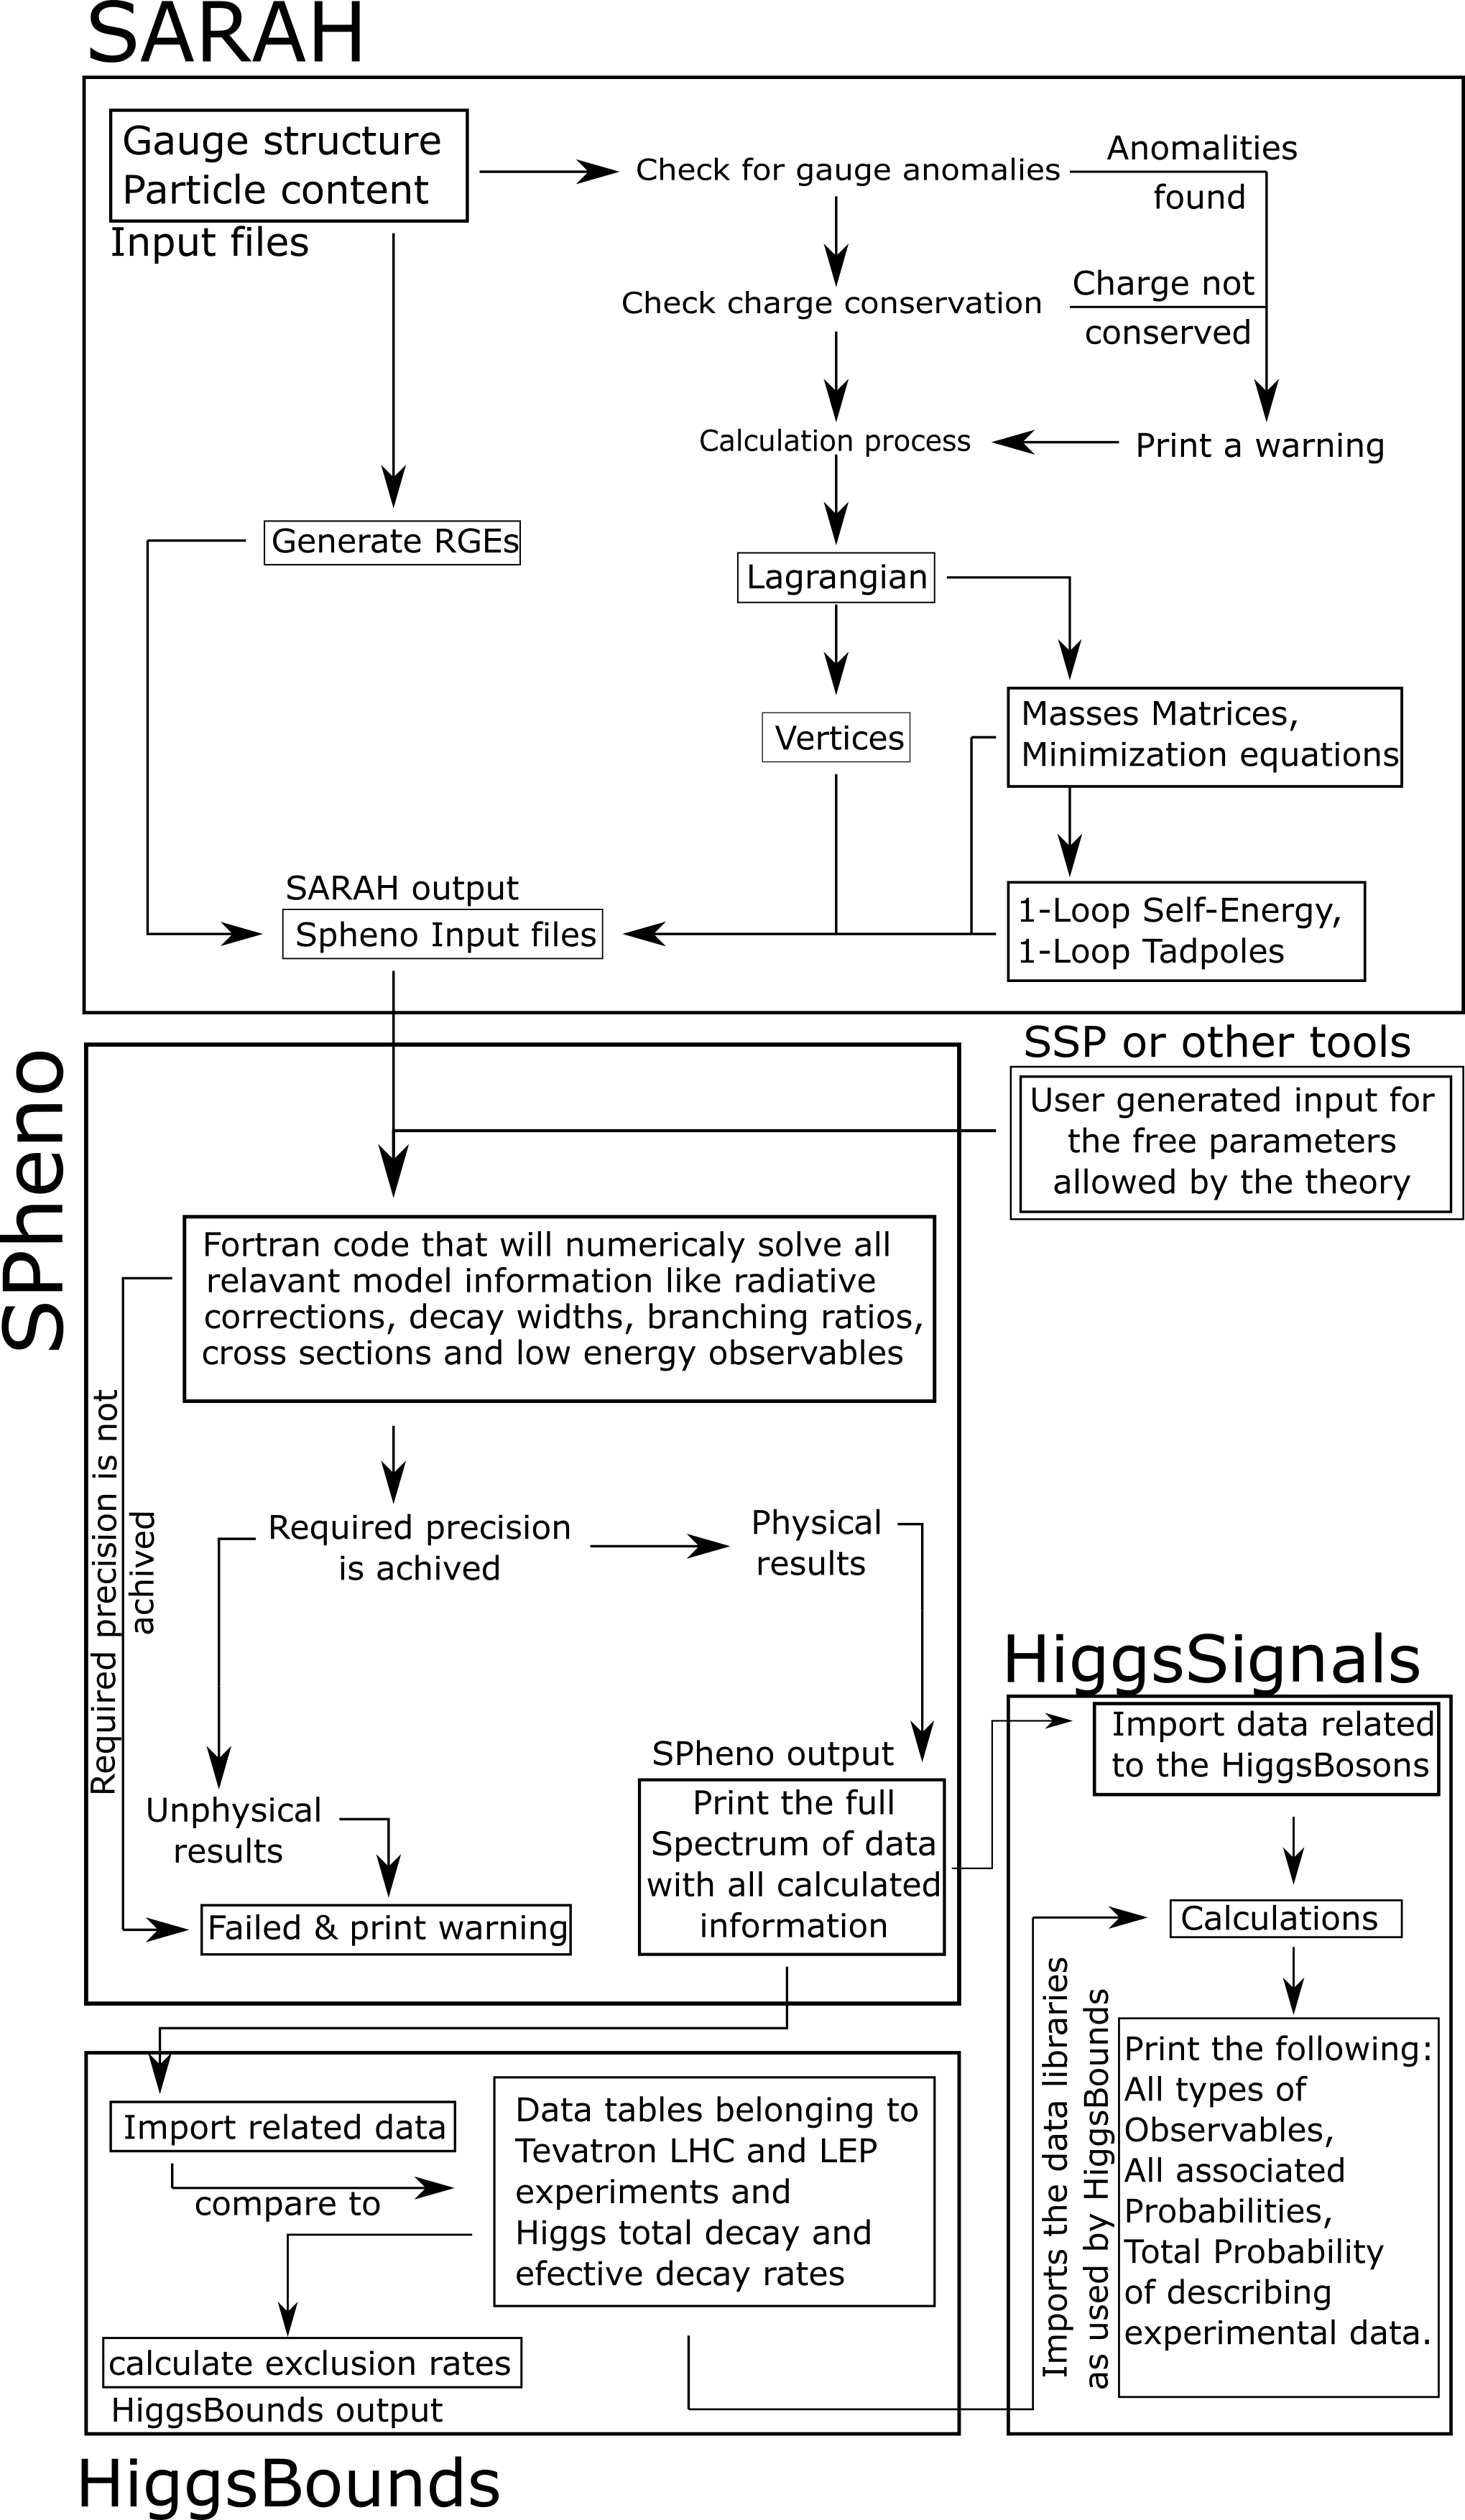
\includegraphics[width=\textwidth , height=22.5cm,keepaspectratio]{shizzle.png}
\caption{A box diagram showing in schematic form the procedure and for the computer calculation of model observable and the program chain}
\label{Prog}
\end{figure}

\subsection{Results}
\subsubsection{Higgs Sector Search}

Now that we've seen and discussed how mass is generated in both the SM and in the B-L-SM model, we find ourselves ready to investigate the viability of our model using the computer tools we just approached in the discussed fashion. 

We begin by re-examining the mass eigenstates seen in the equations (\ref{massa1}) and (\ref{massa2}) we could define and then study a region where the Higgs boson mass would be equal to 125.09 GeV, the observed value. 
%
First, note that the masses of both physical scalars is dependent on 5 parameters, say, $m_{h_1}(\lambda_1,\lambda_2,\lambda_3,v,x)$  One of these parameters, the Higgs VEV, is fixed to $v=175 \sqrt{2} \approx 247$ GeV, then, if we further fix $x = 1000$ GeV we can visually study the behaviour of the scalar masses against the quartic couplings $\lambda_i$.
%
%Consider however that the Higgs mass depends on 5 parameters, the 3 field couplings ($\lambda_1$,$\lambda_2$,$\lambda_3$) and the electroweak and "new" field $\chi$ VEV, being possible to think of the Higgs mass at tree level as a function, , this makes parametrization a issue in 3D space and gives us a few too many variables to study properly using Spheno.
% 
%Given this, to allow for a parametrization in 3D space and being that the most interesting variables to be examined are the potential couplings we will have to define a value for $v$ and $x$,  values used for our first discussion were, $v \approx 246 $ GeV and $x=1000 \; $ GeV.
%
However, note that this is only a tree-level expression and numerical deviations are expected once quantum corrections, built into SPheno, are accounted. In fact this is observed in Fig. (\ref{fig:conic}). While on the left panel, Fig.  (\ref{fig:Teorico}), we represent a surface of $m_{h_1} = 125$ GeV against $\lambda_{1,2,3}$, scanning this surface with Spheno we see on the right panel significant deviations from this value coming just from 1-loop corrections on the mass of the SM like Higgs boson of this model. Note that, in this qualitative analysis, quantum corrections tend to be larger for $\lambda_1$ values without mixing and low  $\lambda_2$ values.
%
\begin{figure}[H]
  \centering
  \minipage{0.49\textwidth}
  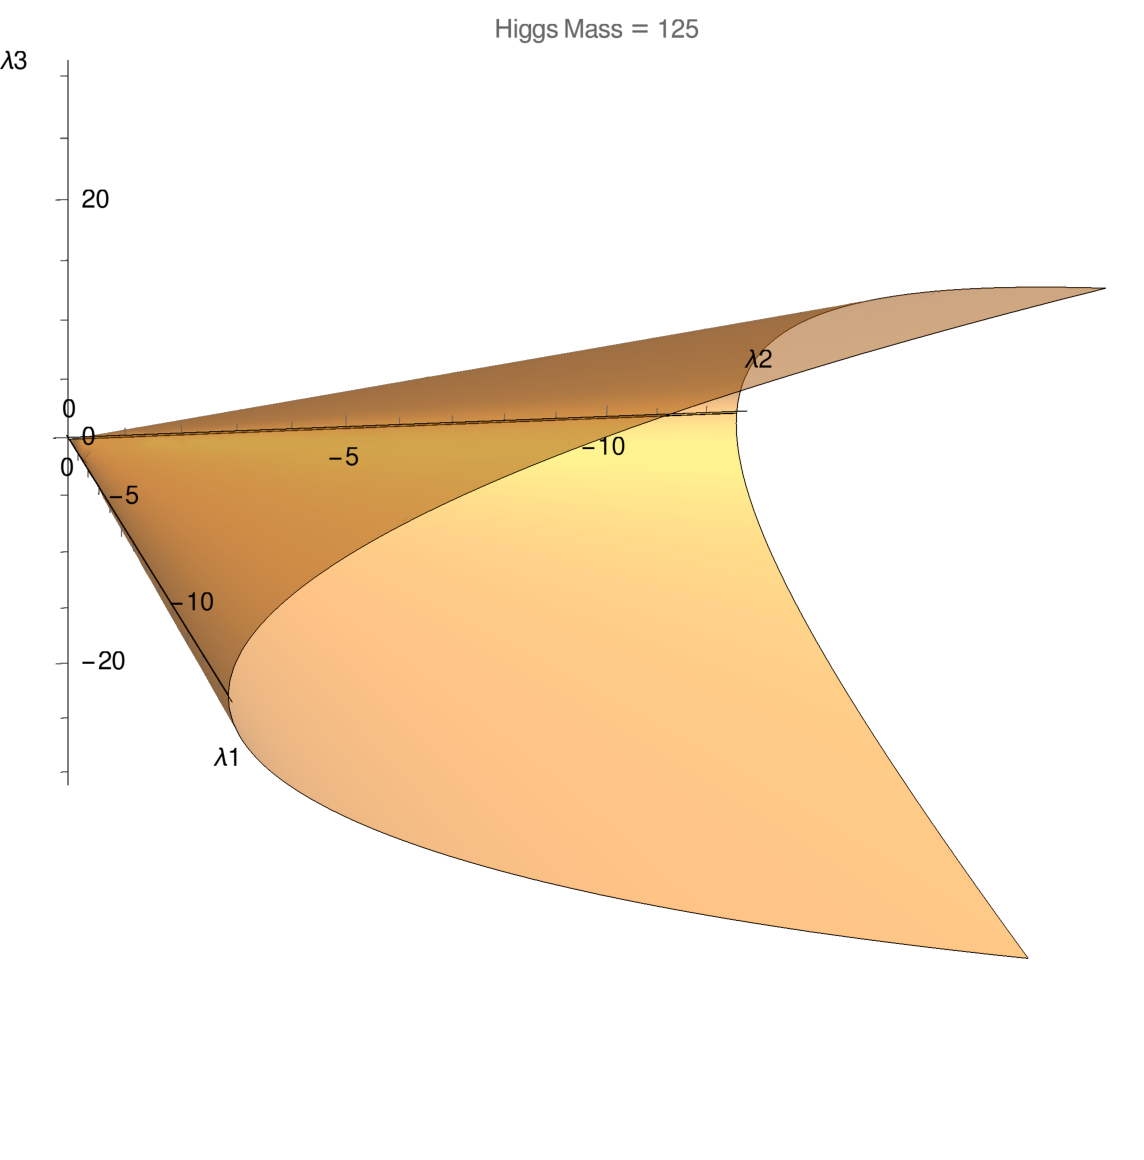
\includegraphics[width=\linewidth,height=7cm,keepaspectratio]{invertido.pdf}
  \caption{A theoretical parametrization of fold where at tree level the higgs mass would be 125.}\label{fig:Teorico}
  \endminipage\hfill
  \minipage{0.49\textwidth}
  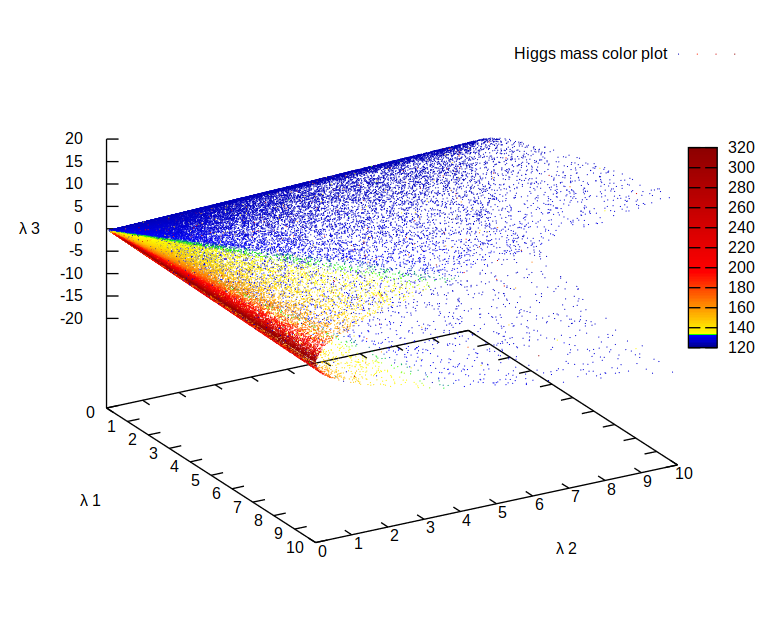
\includegraphics[width=\linewidth,height=7cm,keepaspectratio]{cone.png}
  \caption{1-loop corrections for a tree-level 125 GeV Higgs mass.}\label{fig:conic}
\endminipage\hfill
\end{figure}
%
It can also be seen, on fig. \ref{fig:conic}, that there is a green (dim) line where all points are inside the correct Higgs mass range, i.e. $125.09 \pm 0.21$, meaning that the tree-level contributions are not dominant in that region or somehow cancel out.
%
For the Higgs prime mass we note that its mass grows with $\lambda_2$ indicating that this is the dominant parameter defining the mass of the new scalar Higgs Prime.
%
In fact, as a first approach, we can look again to the respective tree-level expressions Eq. (\ref{massa2})  and observe that, for $v \ll x$, we have
%
\begin{equation}
m_{h_2}^2 \approx x^2 \lambda_2^2 + \sqrt{(-x)^2 \lambda_2} + \sqrt{x v \lambda_3} \approx  2 x^2 \lambda_2^2 
\end{equation}
%
%
which explains why the new scalar mass is mostly sensitive to $\lambda_2$
%
Both these conclusions are taken from the following, now logarithmic scale plots seen in fig. \ref{fig:logh1} and \ref{fig:logh2}, here figure \ref{fig:logh1} is equivalent to figure \ref{fig:conic} in a different scale. 
%
\begin{figure}[H]
  \centering
  \minipage{0.49\textwidth}
  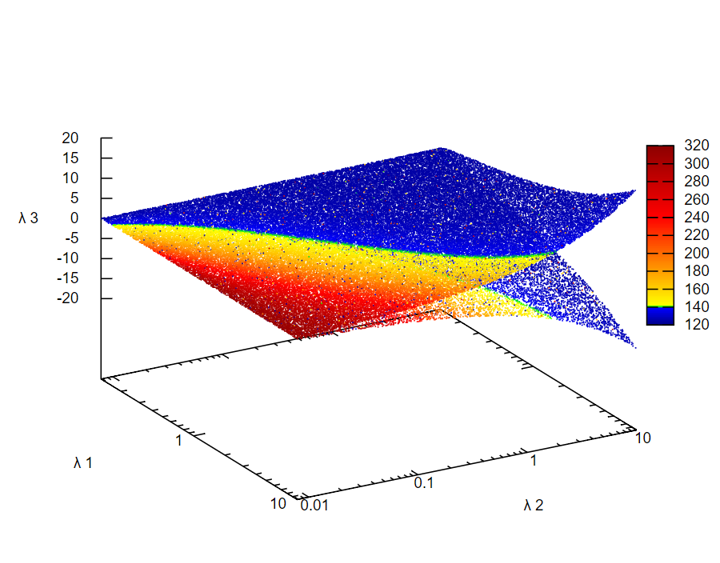
\includegraphics[width=\linewidth,height=6.5cm,keepaspectratio]{Logh11cone.png}
  \caption{A logarithmic representation of the formely Higgs Boson Scan trough a pallete color code in GeVs.}\label{fig:logh1}
  \endminipage\hfill
  \minipage{0.49\textwidth}
  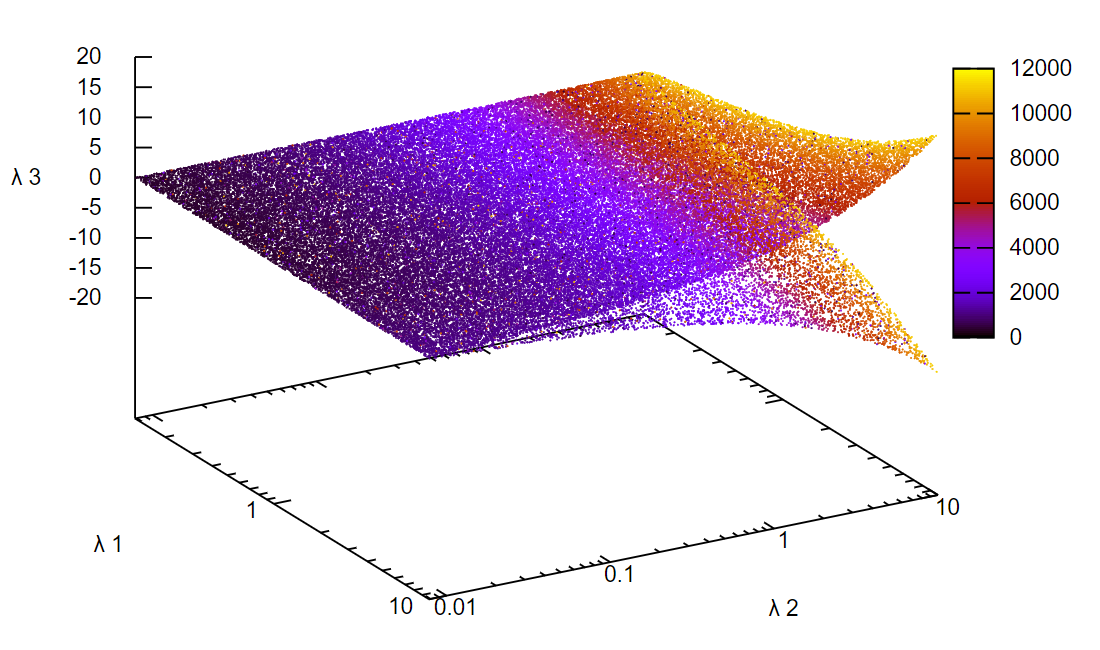
\includegraphics[width=\linewidth,height=6.5cm,keepaspectratio]{Logh2cone.png}
  \caption{The corresponding Higgs Prime boson mass along the same parametrization as seen in fig. \ref{fig:logh1} in GeVs.}\label{fig:logh2}
\endminipage\hfill
\end{figure}
%
Looking closer into these millions of points we find a plane of correct mass region where the Higgs boson mass is within the $125.09 \pm 3$ GeV. We show such points in Fig. \ref{fig:masscerta}. This seemingly indicates that the SM like Higgs Boson is not heavily influenced by quantum corrections up to a cut off point.

\begin{figure}[H]
 \centering
  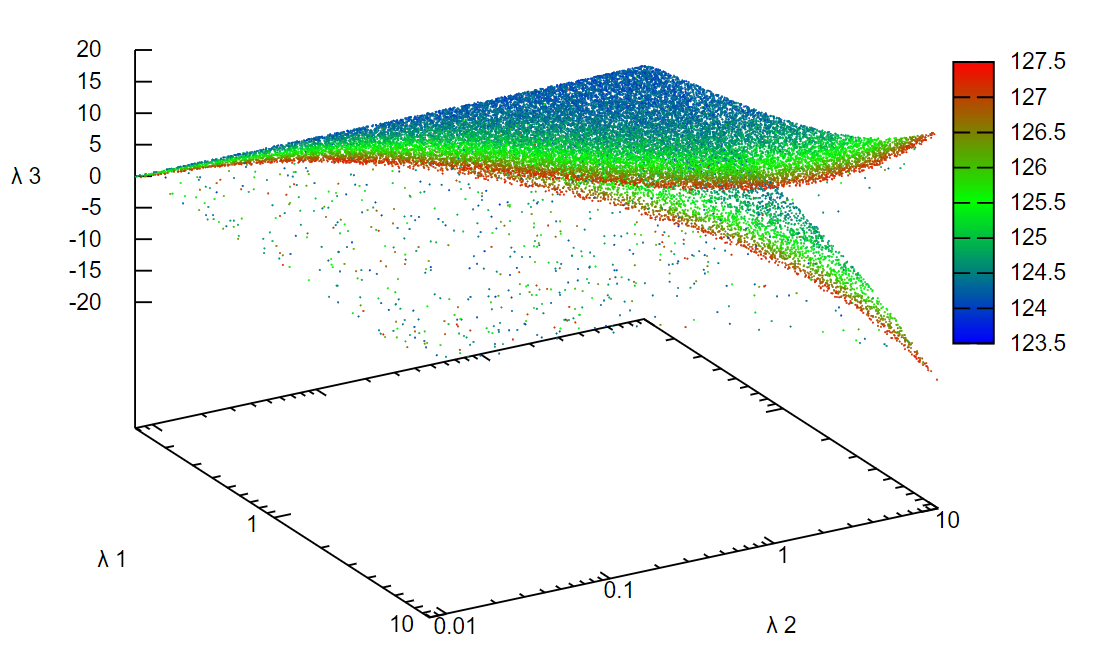
\includegraphics[width=\linewidth,height=7cm,keepaspectratio]{masscert.png}
  \caption{A selection of points where the Higgs Boson Mass was found to be within a 3 GeV interval of the observed 125.09 result.}\label{fig:masscerta}
\end{figure}  
%
The next step was  dedicated to increase the accuracy in the calculation of the Higgs mass by including 2-loop corrections and other miscellaneous corrections. We used the ARGUS computing power and run over several days in order to maximize the amount of data.
%
\begin{figure}[H]
\minipage{0.49\textwidth}
  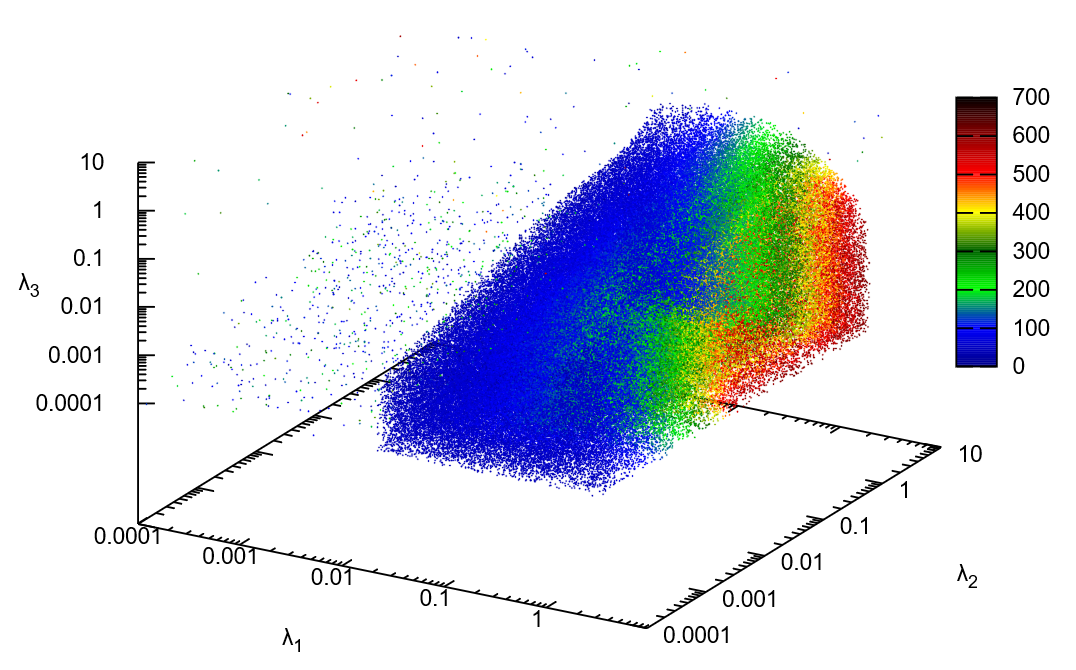
\includegraphics[width=\linewidth]{h1-random-scan.png}
  \caption{A random scan palette plot of the SM Higgs boson Mass where a viable spectrum was outputed by SPheno with 2 loop corrections.}\label{fig:dadosfixes}
\endminipage\hfill
\minipage{0.49\textwidth}%
  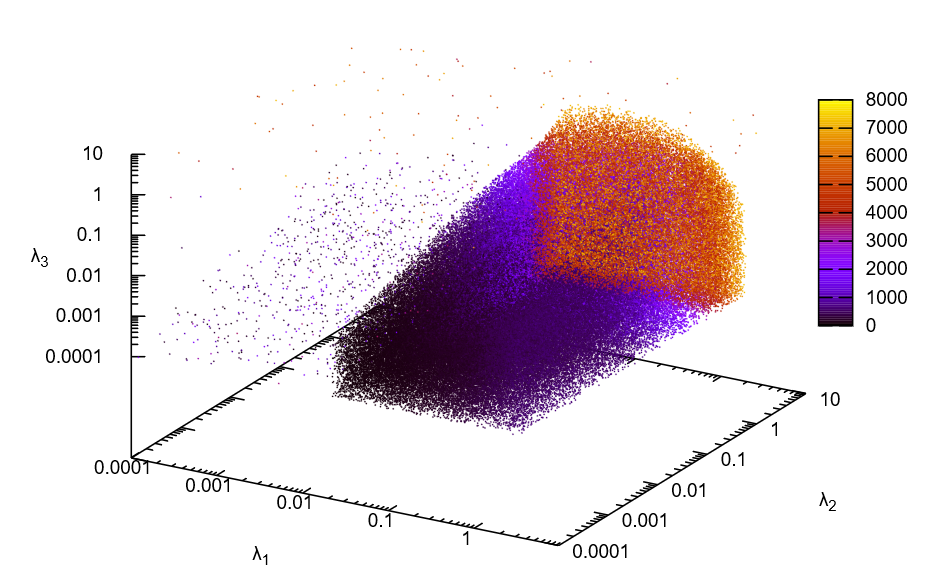
\includegraphics[width=\linewidth]{h2-random-scan.png}
  \caption{A random scan palette plot of the new Higgs Prime boson Mass with 2 loop corrections.}\label{fig:outrosdadosfixes}
\endminipage
\end{figure}
%
%
The following scans were made under a uniform random logarithmic distribution for the $\lambda_i$ couplings between the values of $10^{-4}$ up to $5$ in fact, we know that loop corrections are formally a perturbation expansion on the couplings, which is only well defined around small values of the couplings. It is then possible that 2-loop contributions diverge for larger values of $\lambda_i$. However, a full understanding of this behaviour requires a good knowledge of quantum field theory, which is well beyond the scope of this essay. Our unfiltered after turning on 2-loop correction our random scan results are shown in fig. \ref{fig:outrosdadosfixes} and \ref{fig:dadosfixes}. 
%
%but SPheno now with 2 loop corrections also has convergence conditions that made some points, namely the ones where any the couplings were larger 1 from being viable while some ranges had negative masses that prevented them from forming a physical particle spectrum, these combined led to the shape of the graphics we see bellow. 
%
The same observations as for the 1-loop case hold but now within a range of values for the quartic couplings limited from above by $\lambda_i \sim 1$ to always be approximately in between the 0.1 and 1 scale. 
% 
Once again, we select those points that lie within some deviation from the central value for the Higgs boson mass and show them in Fig. \ref{gaiboi}
%
\begin{figure}[H]
\centering
  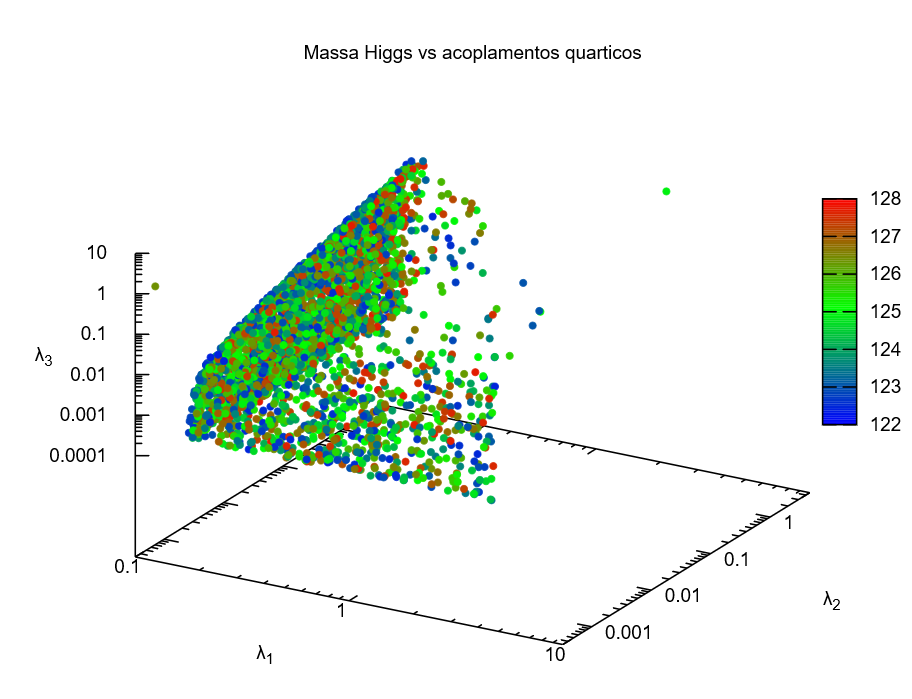
\includegraphics[width=\linewidth,height=7cm,keepaspectratio]{h1shape2loops.png}
  \caption{A palette plot of a selection of points where the SM Higgs Boson mass was found to be within a range of 3 sigma between the values of 122.5 and 127.5 GeVs.}
 \label{gaiboi}
\end{figure}
%
Here we see that again quantum corrections seem to keep the Higgs mass around the tree-level value up to a point seemingly again mainly defined by $\lambda_2$ where they start having a massive impact. 

We can now test the phenomenological viability of these points by running the HiggsBounds and HiggsSignals packages on each of them.

In fig \ref{fig:imnotimportant} we show the Higgs boson mass versus the exclusion ratio given by HiggsBounds. In Fig. \ref{fig:honor} we show a different projection where the observation ratio is plotted against the new Higgs prime mass. In simple terms, if the exclusion ratio is larger than 1 the point is excluded by experimental data. In fact, it means that such a parameter point is predicting a signal larger than the observed limits. On the contrary, if this ratio is smaller than 1, the point is viable. In these two figures, we see that all viable points correspond to an observation ratio larger than 0.6 and, most of them, above 0.85. This means that such points are still valid but either close to rejection or to the discovery of a new scalar particle. It is also interesting to note that, as expected, if we move away from the central Higgs mass, a smooth line shows that the model is no longer as viable. However, there is no clear correlation observed for the Higgs prime mass.

\begin{figure}[h]
\minipage{0.49\textwidth}
  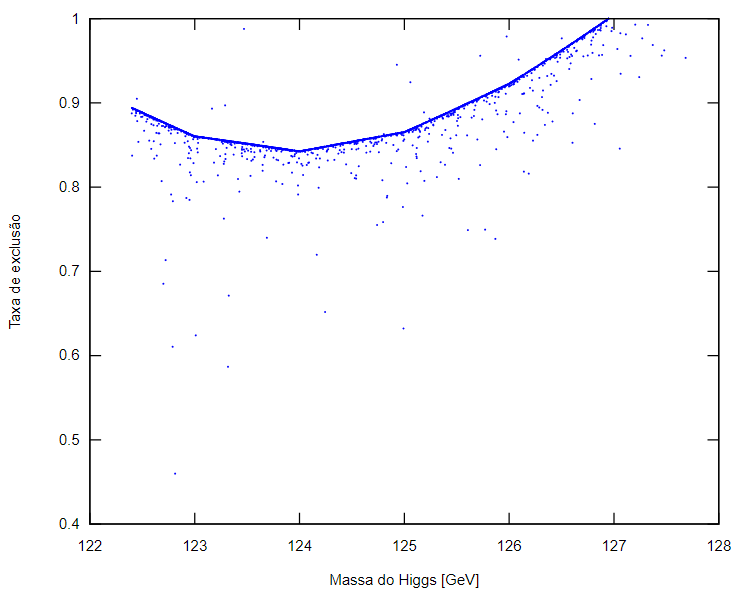
\includegraphics[width=\linewidth]{h1exc.png}
  \caption{A plot of a selection of non excluded SM Higgs boson mass vs the outputed HiggsBounds exclusion  ratio.}\label{fig:imnotimportant}
\endminipage\hfill
\minipage{0.49\textwidth}%
  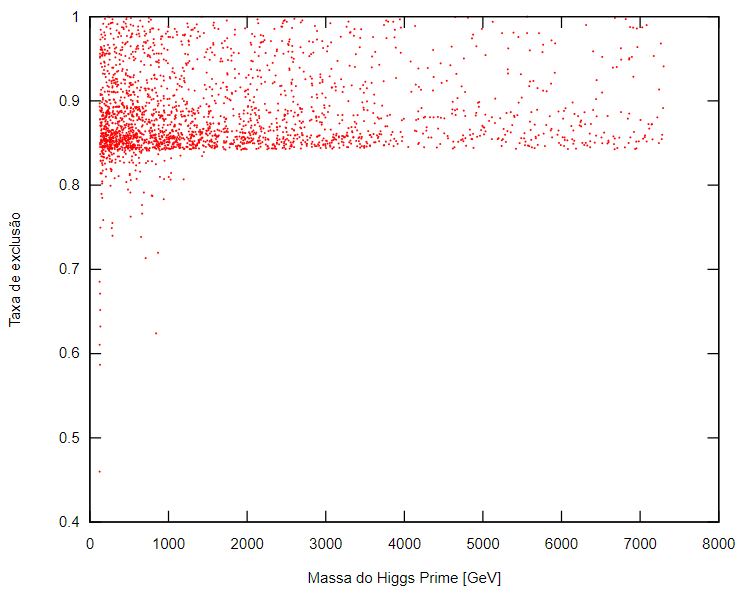
\includegraphics[width=\linewidth]{h2exc.png}
  \caption{A plot of a selection of non excluded Higgs prime boson mass vs the outputed HiggsBounds exclusion ratio.}\label{fig:honor}
\endminipage
\end{figure}

In Figs. \ref{sig1} and \ref{sig2} we show what is denoted the Pvalue against the Higgs and Higgs prime masses respectively. The Pvalue is a parameter calculated by HiggsSignals that tells how well the Higgs boson is reconstructed in each point. It is then without surprise that we see a Pvalue close to 1 at about 125.40 GeV and quickly dropping below 124 GeV or above 126.5 GeV. Note also that, as expected, the Higgs prime mass does not have any impact on this value.

\begin{figure}[H]
\minipage{0.49\textwidth}
  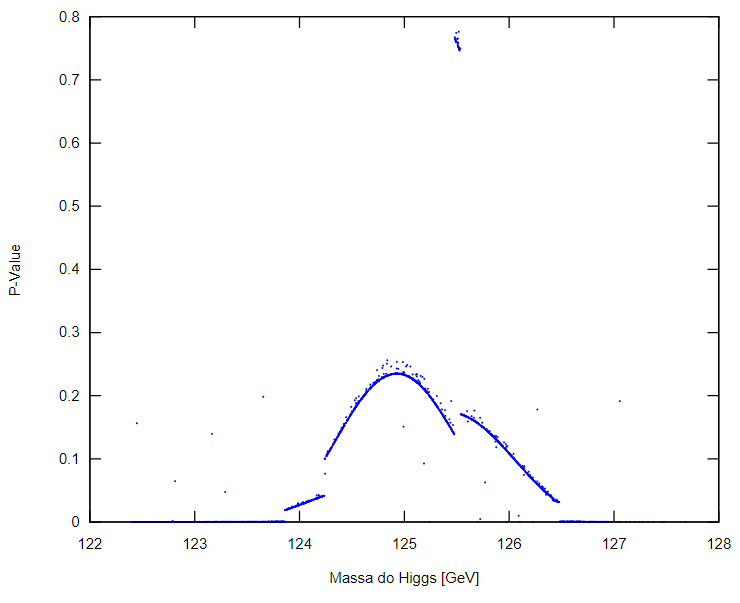
\includegraphics[width=\linewidth]{Pvalh1.png}
  \caption{Exclusion rate vs Higgs mass for the allowed points.}\label{sig1}
\endminipage\hfill
\minipage{0.49\textwidth}%
  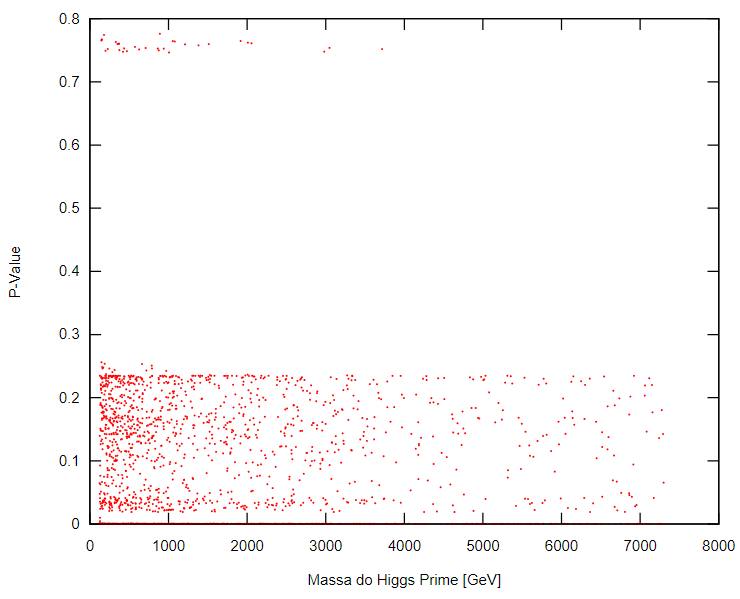
\includegraphics[width=\linewidth]{Pvalh2.png}
  \caption{Exclusion rate vs Higgs prime mass for the allowed points.}\label{sig2}
\endminipage
\end{figure}
 combining these plots in a color palette plot we see, 
\begin{figure}[H]
\centering 
  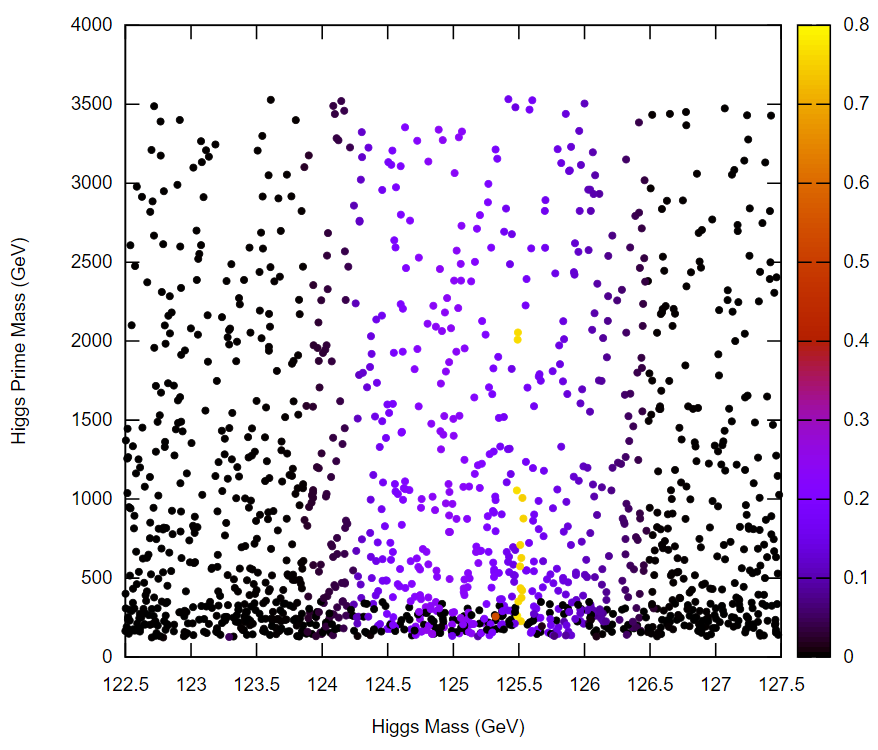
\includegraphics[width=\linewidth,height=7cm,keepaspectratio]{h1vsh2vsobs.png}
  \caption{A pallete plot of the probabilty factor vs the Higgs boson and Higgs prime boson.}\label{fig:awesome_image1}
\end{figure}

%Combining the exclusion given by Higgs and SIgnals a new plot of our Higgs mass and the possible values of the Higgs Prime mass in function of the potential couplings would look something like, 

The points that survived the HiggsBounds exclusion for a viable new scalar and that explain the Higgs boson signal up to to 3 standard deviations are shown in Fig. 17. We see that there is a viability region where all points with small $\lambda_2$ are rejected but only points with small $\lambda_1$ (from 0.12 up to 0.13) are accepted.

\begin{figure}[H]
\centering 
  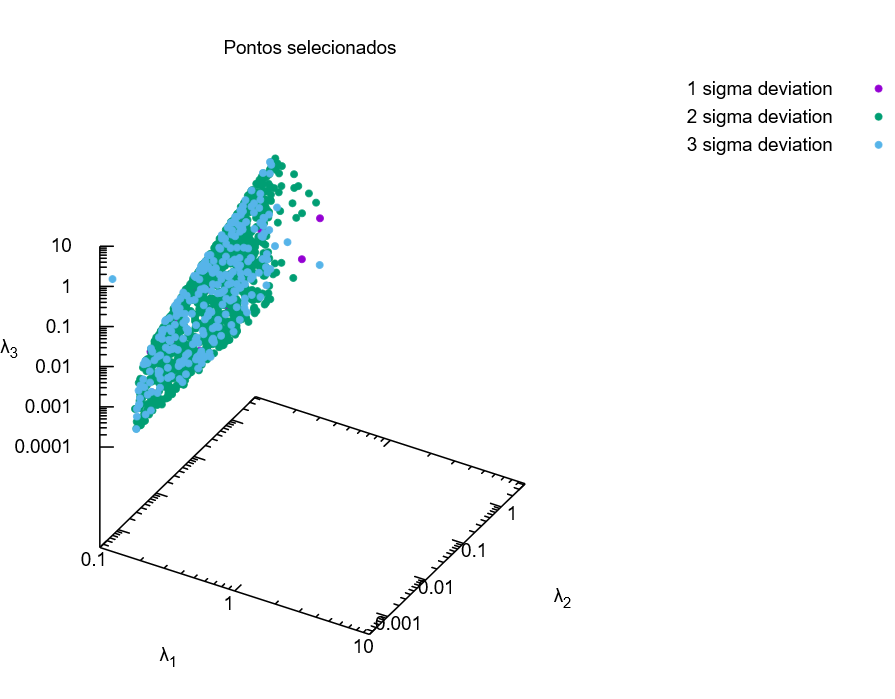
\includegraphics[width=1\linewidth]{signals.png}
  \caption{The quartic couplings points that led to a probability value within a deviation of 1 to 3 $\sigma$ factor.}\label{fig:awesome_image3}
\end{figure}



\subsubsection{The Z' boson} 
\begin{comment}
%As we mentioned in our discussion of the Gauge sector we saw that the equation that gave us the mass of the new gauge zed boson was given by \ref{Gauge zed mass}. 

%This is expression could be written as a function of 4 gauge couplings. One of witch the one related $g$ is strictly a internal parameter in the SPheno calculations and as such we will notbe able to study it.

%Remember SPheno will use this coupling to ensure the correct masses for the low energy observables in the gauge sector.  

This being said we still have 3 gauge coupling parameters that we are in full control. The new $B^\prime_\mu$ coupling, $g^\prime_1$ the SM's $B_\mu$ coupling, $g_1$,  and the kinetic mixing coupling $\tilde{g}$.

A first examination of eigenstates reveal that the main contribution for the Z prime mass will undoubtedly be dominated by the $g^\prime_1$ coupling this because unlike the other terms that have a 1 factor given the $x$ vev being a order of magnitude above the electroweak vev $v$ plus the factor of 16 makes the $g^\prime_1$ coupling have a contribution at of at least two magnitudes more than the other couplings, this means the other couplings will only have  a effect if we limit the $g^\prime_1$ coupling.

However for the SM's Z boson this contribution will mainly be suppressed by the fact the second term would be negative and both have the same of factors  $g^\prime_1$. This allows for a good range of values in all couplings since the mixing angle $\gamma^\prime$ will always be very small due to the fact the $x$ VEV is in the TeV scale. 

Beginning our study now first we assumed no kinetic mixing by setting $\tilde{g}$ to 0 and observed only how the $g_1$ affected the zed prime mass as we varied the $g_1^\prime$ coupling as seen in \ref{Linscaleg1} and \ref{Logslcaeg1} in log scale. 

What we noticed is that the system behaves in somewhat the same fashion tending to the same linear behaviour across $g_1^\prime$ after it takes values larger than 0.1 and that the changing of $g_1$ only offsets the initial value of the Z prime boson.

\begin{figure}[H]
\minipage{0.49\textwidth}
  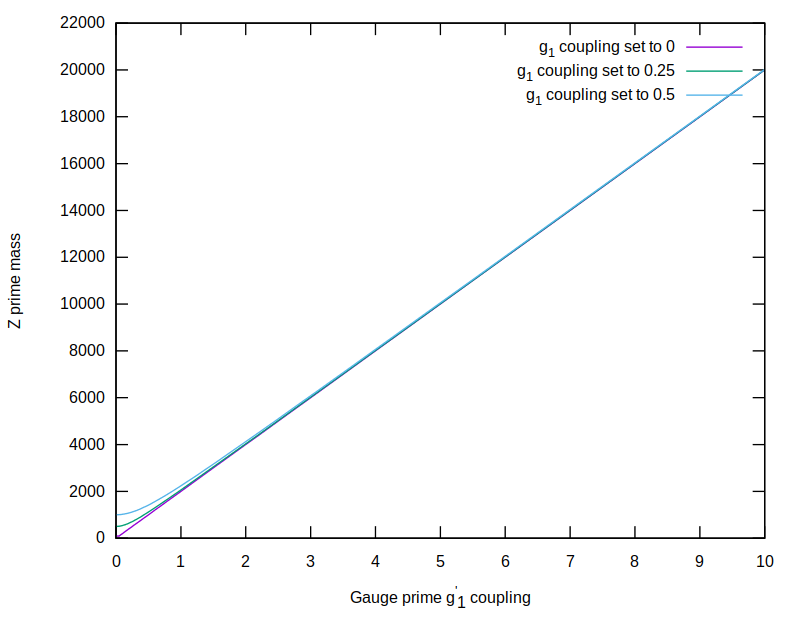
\includegraphics[width=\linewidth]{g1coupling.png}
\label{Logslcaeg1}
\endminipage\hfill
\minipage{0.49\textwidth}%
  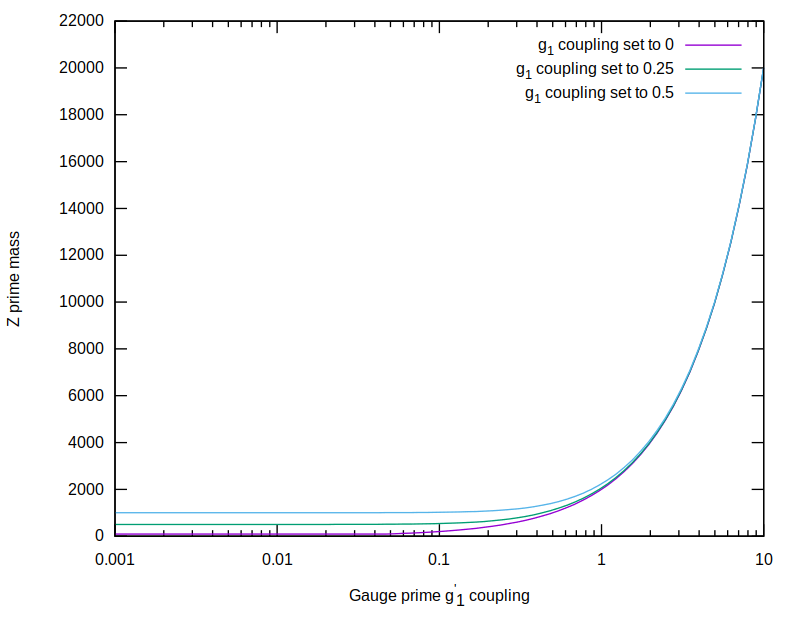
\includegraphics[width=\linewidth]{g1couplinglog.png}
\label{Linscaleg1}
\endminipage
  \caption{Several plots for a different SM gauge couplings in normal and log scale}
\end{figure}

Later we set out to see what type of effect the kinetic mixing coupling $\tilde{g}$ had, to do so we set the gauge coupling $g_1$ to a constant value and tried to observe behaviour changes, the results \ref{tilde1} and \ref{tildel2} show that $\tilde{g}$ has a negligible effect on the Z prime boson mass. 

\begin{figure}[H]
\minipage{0.49\textwidth}
  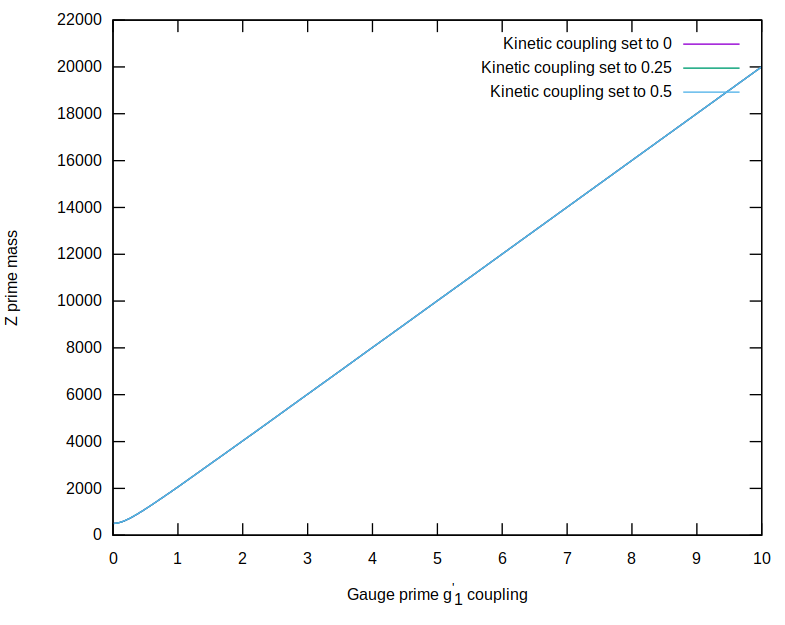
\includegraphics[width=\linewidth]{gtidel.png}
  \label{tilde1}
\endminipage\hfill
\minipage{0.49\textwidth}
  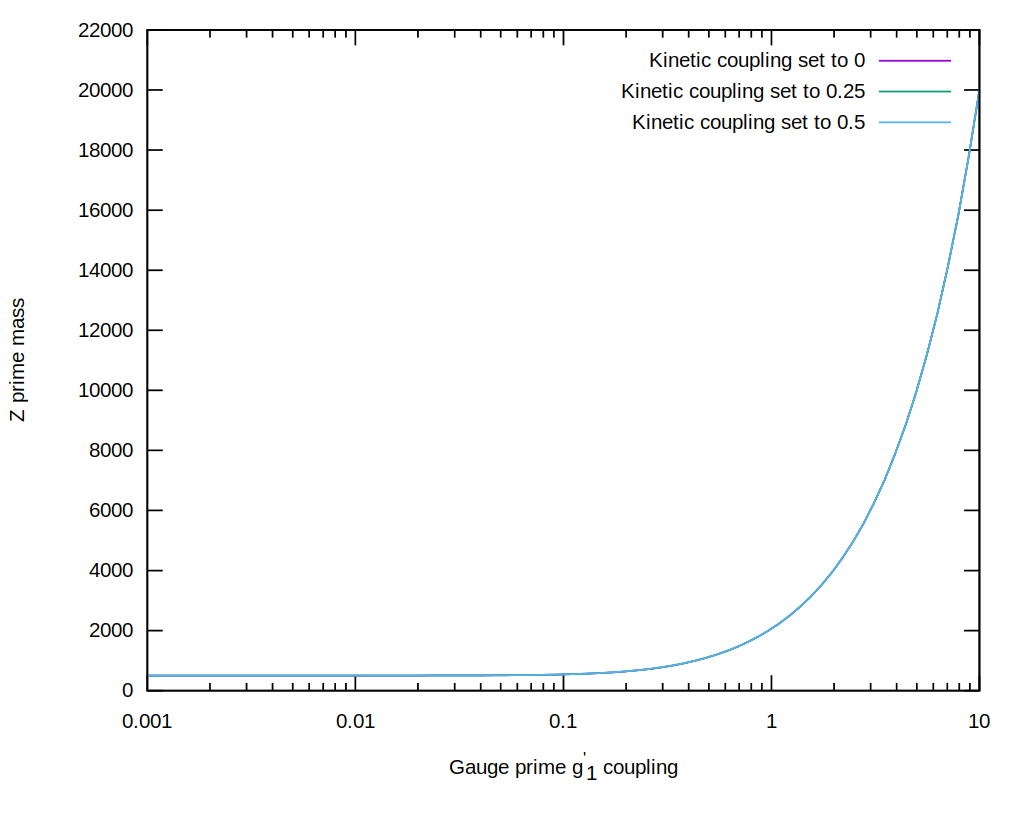
\includegraphics[width=\linewidth]{g1tildlelog.png}
 \label{tildel2}
\endminipage\hfill
\caption{A plot of several gauge coupling scans for different values of kinetic mixing in normal and log scale}
\end{figure}


Has such we can conclude that the only parameter that has a considerable impact is the $g^\prime_1$ coupling. 

Checking experimental data shows that 95 \%  exclusions contrains at ATLAS exotic gauge boson mass has been reached for the Z prime mass under $4.5$ TeV's. \cite{Aaboud:2017buh}


Since any other gauge coupling effects have barely any effect for Z prime mass at that scale we can roughtly say that due to the \ref{massazaprox}
that the gauge coupling range, 

\begin{equation}
M_{Z^\prime \; min} \approx 2 g^\prime_{1 \; min} x  \rightarrow \frac{4.5 \cdot}{2 x} \gtrapprox g^\prime_{1 \; min}
\end{equation}
\end{comment}

%Witch given the TeV scale of x means we could state that the gauge coupling prime has to be greater than 2, %in fact all this data was done with the $x$ VEV set to 1000 to illustrate exactly that. 

As it was already discussed, the requirement of a large $x \gg v$ implies that the Z' mass is decoupled from the SM Z boson and essentially depends on $g_1^\prime$ and x. Searches for Z' bosons in the B-L-SM were already performed by ATLAS and are reported in
\begin{table}[h]
\centering
\begin{tabular}{|c|c|c|c|c|c|c|}
\hline
Model                             & \multicolumn{6}{l|}{Lower limits on}                                                                           \\ \hline
\multirow{3}{*}{$Z^\prime_{B-L}$} & \multicolumn{2}{l|}{$ \quad \; ee$} & \multicolumn{2}{l|}{$\quad \; \mu \mu $} & \multicolumn{2}{l|}{$\quad \; l \; l$} \\ \cline{2-7} 
                                  & obs        & exp        & obs                          & exp                         & obs        & exp        \\ \cline{2-7} 
                                  & 4.0        & 4.0        & 3.6                          & 3.6                         & 4.2        & 4.1        \\ \hline
\end{tabular}
\caption{Experimental limits on the Z prime boson}
\label{shit}
\end{table}

In particular, the most stringent limit is coming from the decay into electrons, $Z' \rightarrow e e$, where the Lower limit in the Z' mass is 4.0 TeV at 95 \% confidence level as seen in table \ref{shit}. 
This means that 
$M_{Z' \text{min}} \simeq 2 g_1^\prime x \Rightarrow x_{\text{min}} \simeq  \frac{4}{ 2 g_1^\prime}  \; \text{TeV} \Rightarrow  x_{\text{min}} \simeq \frac{2}{g_1^\prime} \  \text{TeV}$.
Then, for our choice of x in the previous section, recall $x = 1$ TeV, it implies that the gauge coupling should be $g_1^\prime = 2$ for our model points not being excluded. We also see that if we were to choose $ g_1^\prime = 1$, $0.5$ and $0.1$, the minimum values of x would be 2 TeV, 4 TeV and 20 TeV respectively. As a future study it would be interesting to study the impact of larger VEVs in the masses and observation ratios of the new scalar $h^\prime$  \cite{Aaboud:2017buh}. 

\newpage
 

\subsection{Conclusion} 
We began this essay by studying the SM and saw just how effective it can be at describing particle interactions up to the electroweak energy scale and how in the SM the mechanism behind mass generation stems from the breaking of a symmetry $SU(2) \times U(1)$ symmetry. We noted its inability to produce mass for neutrinos and this led us to explore the B-L-SM model, a extension of the SM that allowed to solve these issues. We used a minimal extension by means of a new Abelian gauge $U(1)_{B-L}$ symmetry and the introduction of right handed neutrinos. To break the $U(1)_{B-L}$ we also added a complex singlet whose VEV is responsible for generating mass to a new Z' gauge boson, a new scalar particle as well as three light and three heavy neutrinos. for right handed neutrinos and massive left handed neutrinos. We saw this model added a new $Z^\prime$ boson and  new scalar particle Higgs particle. 

We explored computer tools that allow for a study of the viability for our model. We gave the new gauge field $\chi$ a VEV of 1 TeV we discovered it to be far too low for a non-perturbative theory like quantum field theory to likely explain the Z prime boson, however for it we found a possibly viable range for the self interaction and cross interaction couplings of  the scalar sector of the B-L-SM model.

We have thoroughly studied the scalar sector and its phenomenological viability in terms of accurately reproducing the Higgs mass and predicting a new scalar. We have studied the impact of one and two-loop corrections to the Higgs sector and verified that in the later case the quartic couplings in the scalar potential become limited from above with the maximum value $\lambda_i = 1$. We have also required that for all viable model points that we studied the Z' mass was 4 TeV and hence the $g_1^\prime$ coupling had to be equal to 2.

As a future work, it would be interesting to let the singlet VEV x vary and, while imposing an allowed mass for the Z' gauge boson, study the effect of x on the viability region found in Fig. 17. It would also be interesting to perform phenomenological studies on the three heavy neutrinos and understand whether they could be observable or not at collider experiments. 
This model would also allow for a mass study of the neutrino mass spectrum based on the variation of yukawa couplings. 

\newpage 
\section{Appendix}
\subsubsection{Notation, Relativity and Lorentz transformations}

Since the focus of this essay approaches the analysis of quantum theories that are tied to particle physics at the electroweak scale and beyond, we must ensure our study must be consistent with the theory of special relativity. Therefore we must revisit the definitions, the notation and the representations used in relativistic theories. From here onwards we will use natural units, so consider $\hbar=c=1$. This gives all quantities dimensions of mass to some power.

Starting off shallowly touching on some basic concepts of relativity. Starting with the notion of interval between two events, this notion will replace our previous understanding of distance in a frame of motion. 

For a generic set of space-time coordinates the interval between them is the quantity,$s$ and is defined by $s^2=c^2 dt^2 - (dx^2 +dy^2 + dz^2) $. This configuration of signs is stipulated by convenience, it would still be equivalent to have the plus and minus signs swapped but we will use the mostly negative representation during this essay.



\begin{align}
x^\mu= & (x^0,x^1 ,x^2 ,x^3) = (-ct,x,y,z)  \\  x_\mu= & (x_0,x_1 ,x_2 ,x_3) = (ct,-x,-y,-z)  
\end{align}
We also define the covariant differential operator as a vector in this notation: 

\begin{equation}
\partial_\mu = g_{\mu \nu} \partial^\nu = (\partial_0,\partial_1 ,\partial_2 ,\partial_3)=(\frac{1}{c} \frac{\partial }{\partial t },\frac{\partial }{\partial x },\frac{\partial }{\partial y },\frac{\partial }{\partial z })=(\frac{1}{c} \frac{\partial}{\partial t} , \nabla)=\frac{\partial}{\partial x^\mu}
\end{equation}

In this notation a vector with a upper index is called a covariant index and a vector with a lower index is called a contravariant vector. The inner product of these vectors would as we mention be a Lorentz invariant scalar. To further simplify the notation we will be combining this with the summation convention so a "contracted" index will automatically be summed from 0 to 3 as shown 

\begin{equation}
\sum_{\mu=0}^{3}  V_\mu V^\mu \longrightarrow V_\mu V^\mu
\end{equation}

The relation relation between covariant and contravariant vectors is expressed with auxiliary to the space metric, $\eta_{\mu \nu}$. \cite{ryder1996quantum}

\begin{align} 
x_\mu & =  \eta_{\mu \nu} x^\nu  \\ 
x_\mu & =  \eta_{\mu 0} x^0  + g_{\mu 1} x^1  + g_{\mu 2} x^2 + g_{\mu 3} x^3  
\end{align}
\newpage
\bibliographystyle{unsrt}
\bibliography{References_old}


	

\end{document}
